\documentclass[a4paper, 11pt]{article}
\usepackage[italian]{babel}
\usepackage[utf8]{inputenc}
\usepackage{amsmath}
\usepackage{imakeidx}
\usepackage{amsfonts}
\usepackage{amssymb}
\usepackage{float}
\usepackage{graphicx}
\usepackage{caption}
\usepackage[paper=a4paper]{geometry}
\usepackage[shortlabels]{enumitem}
\usepackage{hyperref}
\usepackage{caption}
\captionsetup[figure]{justification=centering}
% Frontespizio config
\usepackage[nowrite]{front-th}
\usepackage{pdfpages}

\usepackage{fancyhdr} % <-- aggiunto
\pagestyle{fancy}     % <-- imposto lo stile fancy
\fancyhf{}
\rhead{\includegraphics[width=1cm]{Immagini/Logo_Università_di_Udine.png}} % <-- logo in alto a destra
\hypersetup{
    colorlinks,
    citecolor=black,
    filecolor=black,
    linkcolor=black,
    urlcolor=black
}

\setcounter{secnumdepth}{4}
\setcounter{tocdepth}{4}

% --- INIZIO SOSTITUZIONE MINTED CON LISTINGS ---
\usepackage{listings}
\usepackage{xcolor} % Necessario per definire i colori

\definecolor{codegray}{gray}{0.95}
\definecolor{codegreen}{rgb}{0.0, 0.5, 0.0} % Per i commenti
\definecolor{codered}{rgb}{0.9, 0.0, 0.0}   % Per le stringhe
\definecolor{codeblue}{rgb}{0.0, 0.0, 0.9}   % Per le parole chiave

\lstdefinestyle{mycodestyle}{
    backgroundcolor=\color{codegray}, % Colore di sfondo
    basicstyle=\small\ttfamily,       % Stile del testo del codice (dimensione piccola, font a spaziatura fissa)
    breaklines=true,                  % Permette al codice di andare a capo
    frame=single,                     % Aggiunge un bordo singolo
    framesep=5pt,                     % Spazio tra il bordo e il codice
    framerule=0.5pt,                  % Spessore del bordo
    rulecolor=\color{orange!70},     % Colore del bordo (arancione come nel tuo esempio)
    numbers=left,                     % Numerazione delle righe a sinistra
    numberstyle=\tiny\color{gray},    % Stile dei numeri di riga
    stepnumber=1,                     % Incremento dei numeri di riga
    numbersep=8pt,                    % Spazio tra numeri e codice
    showspaces=false,                 % Non mostrare spazi come simboli
    showtabs=false,                   % Non mostrare tab come simboli
    showstringspaces=false,           % Non mostrare spazi nelle stringhe
    commentstyle=\color{codegreen}\textit, % Stile per i commenti (verde, corsivo)
    keywordstyle=\color{codeblue}\bfseries, % Stile per le parole chiave (blu, grassetto)
    stringstyle=\color{codered},      % Stile per le stringhe (rosso)
    % Se vuoi un titolo/didascalia per il blocco di codice, potresti usare captionpos, ad esempio:
    % captionpos=b, % didascalia sotto
    % caption={Descrizione del codice},
}
% --- FINE SOSTITUZIONE MINTED CON LISTINGS ---


\renewcommand{\contentsname}{Indice}

\newcommand{\myfrontpage}{%
  \begin{titlepage}
  \centering
  \preparefrontpage
  \end{titlepage}
  %\global\let\centering\relax % Disabilita centering globale
}

\fontoptionnormal

\makeatletter
\def\front@thecandidate{Candidato}
\def\front@thecandidates{Candidati}
\def\front@theadvisor{Relatore}
\def\front@theadvisors{Relatori}
\makeatother


% Dati frontespizio
\Universita{Udine}
\Logo[3.5cm]{./Immagini/Logo_Università_di_Udine.png}
\Dipartimento{Scienze Matematiche, Informatiche e Fisiche}  % Aggiunto in sostituzione di Facoltà
\Corso[Laurea]{Internet Of Things, Big Data, Machine Learning}
\Annoaccademico{2024--2025}
\Titolo{Laboratorio di Algoritmi e Strutture Dati\bigbreak - \bigbreak Verifica della complessità asintotica degli algoritmi di ordinamento}
\Candidato{Andrea Gioia\\(169484) - 169484@spes.uniud.it}
\Candidato{Luca Gamberini\\(168712) - 168712@spes.uniud.it}
\Candidato{Kent Idrizi\\(168711) - 168711@spes.uniud.it}
\Relatore{Prof. Gabriele Puppis}
\Relatore{Prof. Carla Piazza}
% \Correlatore{Prof. Marco Sciandrone}  % Commentato come richiesto



\begin{document}
\myfrontpage

\thispagestyle{empty} 
%\preparefrontpage

\newpage

\tableofcontents
\newpage
\section{Introduzione}
Il progetto include le misurazioni e la conseguente graficazione di 4 algoritmi di ordinamento:
\begin{itemize}
    \item QuickSort
    \item QuickSort 3 Way
    \item CountingSort
\end{itemize}
\subsection{Specifiche tecniche}
Le specifiche tecniche delle misurazioni sono state:
\begin{itemize}
    \item Array generato con valori decimali \textbf{casuali}
    \item La lunghezza dell'array è compresa tra 100 e 100 mila valori
    \item Il valore di ciascun elemento dell'array varia casualmente tra 10 e un milione
\end{itemize}
Gli algoritmi sono stati implementati in linguaggio Python. \\
Le misurazioni dei tempi sono state acquisite tramite la funzione \href{https://docs.python.org/3/library/time.html#time.perf_counter}{\textit{\texttt{perf\char`_counter}}} della libreria \textit{time}.

\section{Algoritmi}
Gli algoritmi di ordinamento presi in esame presentano caratteristiche differenti e risultano più o meno efficienti in base alle carattestiche dell'array di elementi da ordinare.

\subsection{QuickSort}
Algoritmo di ordinamento ricorsivo del tipo divide-et-impera, quindi basato sulla suddivisione in n sottoproblemi, risolti ricorsivamente, fino al raggiungimento del caso base.\\
Non presenta la necessità di utilizzo di strutture dati aggiuntive, di conseguenza lo scambio di elementi avviene in-place.\bigbreak
\noindent  \underline{Idea} \\ Divide: partizionando l'array A[p:r] in due sottoarray A[p:q-1] (parte inferiore) e A[q+1:r] (parte superiore) in modo che ciascun elemento della parte 
inferiore sia minore o uguale al pivot A[q], il quale è a sua volta minore o uguale a ciascun elemento della parte superiore. Calcolare l'indice q del pivot fa parte della procedura 
di partition. Impera: richiamando ricorsivamente quicksort su ciascun sottoarray A[p:q-1] e A[q+1:r]. Infine per combinare non serve far 
nulla dato che i due sottoarray sono già ordinati, per cui avrò che l'intero sottoarray A[p:r] è ordinato. 
La procedura Partition invece mi permette di stabilire un perno, a quel punto avrò che gli elementi precedenti sono minori del perno mentre quelli a destra saranno maggiori,
considerando però che successivamente vanno ordinati.\bigskip

\noindent Le complessità asintotiche temporali di QuickSort sono: 
\begin{itemize}
    \item Caso ottimo: $\Omega(n\log_2n)$
    \item Caso medio: $\Theta(n\log_2n)$
    \item Caso peggiore: $\mathcal{O}(n^2)$
\end{itemize}

\subsubsection{Analisi delle complessità}
Il QuickSort è un esempio di algoritmo che lavora in-place, quindi la complessità in spazio equivale a $\Theta(n)$, ovvero la dimensione dell'array di partenza.\bigbreak
\noindent Le operazioni che influiscono sulla complessità di tempo sono:
\begin{itemize}
    \item Chiamata a partition, complessità $\Theta(n)$
    \item Le due chiamate ricorsive, complessità rispettivamente di $T(q-1)$ e $T(n-q)$.
\end{itemize}


\noindent L'equazione di ricorrenza di QuickSort è:
\begin{gather*}
    T(n) = 
    \begin{cases}
    \Theta(1)\quad\quad \text{se}\;\; n\; \leq\; 1 \\
    T(q - 1) + T(n - q) + \Theta(n)\quad\quad se\; n > 1
    \end{cases}     
\end{gather*}

\noindent Spiegazione delle complessità:
 
\begin{itemize}

  \item \textbf{Caso migliore:} il pivot divide sempre l'array in due parti, ovvero partition produce due sottoproblemi di dimensione al massimo n/2,
   dato che uno è di dimensione $\lfloor \frac{n-1}{2} \rfloor \leq \frac{n}{2}$ e 
   l'altro di dimensione $\lceil \frac{n-1}{2} \rceil - 1 \leq \frac{n}{2}$. 
   Un limite superiore al tempo di esecuzione è descritto da: $T(n) = 2T\left(\frac{n}{2}\right) + \Theta(n)$
  
  \item \textbf{Caso medio:} ogni possibile posizione del pivot nel caso medio ha probabilità $\frac{1}{n}$ di essere scelta. Per cui tutti i casi sono equiprobabili. 
  Per un input casuale la complessità media è $T(n) = \frac{1}{n}\sum_{i=0}^{n-1}\left[T(i) + T(n-i-1)\right] + \Theta(n)$ che si risolve in
   $\mathbb{E}[T(n)] = \Theta(n \log n)$.

  \item \textbf{Caso peggiore:} quando la partizione produce un sottoproblema con n-1 elementi e uno con 0 elementi. Si può assumere che questa 
  partizione sbilanciata avvenga ad ogni chiamata ricorsiva. La partizione costa $\Theta(n)$. Dato che la chiamata ricorsiva su un array di dimensione 
  0 ritorna senza fare nulla, $T(0) = \Theta(1)$, 
  e l'occorrenza del tempo di esecuzione è $T(n) = T(n-1) + T(0) + \Theta(n) = T(n-1) + \Theta(n)$ con soluzione finale $T(n) = \Theta(n^2)$. 
  Dunque, se la partizione è massimamente sbilanciata in ogni livello ricorsivo dell'algoritmo, il tempo di esecuzione è $\Theta(n^2)$.

\end{itemize}

\noindent Quicksort non è stabile: funziona dividendo l’array in sottosequenze basate su un pivot, e poi riordinando ricorsivamente. 
Durante questo processo: gli elementi uguali al pivot possono finire in posizioni diverse rispetto all’ordine originale; questo accade 
perché lo scambio degli elementi non tiene conto della loro posizione iniziale, ma solo del confronto con il pivot.

\subsubsection{Codice}
\begin{lstlisting}[style=mycodestyle, language=Python]
def QuickSort( A, p, q ):
    if( p < q ):
        r = Partition( A, p, q)
        QuickSort( A, p, r-1 )
        QuickSort( A, r+1, q )
    return A

def Partition(A, p, q):
    x = A[q]
    i = p - 1
    for j in range(p, q):
        if A[j] <= x:   # (corretto A[j], non A[q])
            i += 1
            Scambia(A, i, j)
    Scambia(A, i + 1, q)    # posiziona il pivot al centro
    return i + 1

def Scambia(A, i, j):
    temp = A[i]
    A[i] = A[j]
    A[j] = temp
\end{lstlisting}

\subsubsection*{Funzionamento del codice}

\begin{enumerate}
  \item \textbf{Funzione Scambia(A, i, j):} Lo scopo è scambiare due elementi in un array. A è l'array degli elementi,
   i e j gli indici degli elementi da scambiare. Memorizza temporaneamente il valore di A[i] 
   in temp; Assegna A[j] alla posizione i; Ripristina il valore originale di A[i] (ora in temp)
   nella posizione j. Costo $\mathcal{O}(1)$.

  \item \textbf{Funzione Partition(A, p, q):} Lo scopo è partizionare l'array in modo che tutti gli elementi 
   minori uguali al pivot siano a sinistra e quelli maggiori del pivot a destra. A è l'array da partizionare,
   p l'indice iniziale del sottovettore, q l'indice final (usato come pivot). Si sceglie il pivot x = A[q] (ultimo elemento);
   l'indice i tiene traccia della fine della sezione degli elementi minori o uguali al pivot; il ciclo for scorre l'array da p a q-1, 
   Se A[j] è minore uguale al pivot, incrementa i e scambia A[i] con A[j]; infine scambia A[i+1] (primo elemento maggiore del pivot) con A[q] (pivot). 
   Ora, il pivot è nella sua posizione corretta.

  \item \textbf{Funzione QuickSort(A, p, q):} Lo scopo è ordinare ricorsivamente l'array utilizzando il partizionamento. 
  A è l'array da ordinare, p l'indice iniziale e q l'indice finale. La condizione di base è se $p \geq q$, il sottovettore ha 0 o 1 elemento → già ordinato.
  $r = Partition(A, p, q)$ posiziona il pivot e restituisce la sua posizione finale. QuickSort(A, p, r-1) ordina la parte sinistra 
  (elementi minori o uguali al pivot); QuickSort(A, r+1, q) ordina la parte destra (elementi maggiori del pivot).
\end{enumerate}

\subsection{QuickSort3Way}
QuickSort 3-Way è un'ottimizzazione del QuickSort classico progettata per gestire efficientemente array con molti elementi duplicati.  
Mentre il QuickSort standard partiziona l'array in due sottoarray (elementi $\leq$ pivot ed elementi $> $ pivot), la versione 3-Way divide l'array in tre partizioni:
\begin{itemize}
  \item Elementi minori del pivot (a sinistra).
  \item Elementi uguali al pivot (al centro).
  \item Elementi maggiori del pivot (a destra).
\end{itemize}
A differenza del QuickSort classico, QuickSort 3-Way presenta una notevole efficienza con array contenenti molti elementi duplicati.  
\bigbreak

\noindent  \underline{Idea} \\ Scelta del pivot: Il primo elemento dell'array (arr[l]) è selezionato come pivot.\\
Inizializzazione dei puntatori: \\
- lt (less than): confine sinistro degli elementi minori del pivot.\\
- gt (greater than): confine destro degli elementi maggiori del pivot.\\
- i: puntatore corrente per scorrere l'array.\\
Partizionamento 3-way:\\
- Se $ \texttt{arr[i]} < \texttt{pivot} $: scambia arr[i] con arr[lt], incrementa lt e i\\
- Se $ \texttt{arr[i]} > \texttt{pivot} $: scambia arr[i] con arr[gt], decrementa gt (senza incrementare i).\\
- Se $ \texttt{arr[i]} == \texttt{pivot} $: incrementa solo i.\\
Ricorsione:\\
- Applica ricorsivamente l'algoritmo alle partizioni sinistra (l a lt-1) e destra (gt+1 a r).\\
- La partizione centrale (lt a gt) contiene elementi già ordinati (tutti uguali al pivot).\\
\bigskip

Le complessità asintotiche temporali di QuickSort3Way sono:
\begin{itemize}
    \item Caso ottimo: $\Omega(n\log n)$
    \item Caso medio: $\Theta(n\log n)$
    \item Caso pessimo: $\mathcal{O}(n^2)$
\end{itemize}

\subsubsection{Analisi delle complessità}
Come nel caso di QuickSort, anche il QuickSort3Way lavora in-place, senza bisogno di stutture dati aggiuntive, quindi la complessità in spazio è $\Theta(n)$.\\\\
Considerando che l'algoritmo itera gli elementi dell'array e siccome il ciclo for viene eseguito al massimo $n$ volte.\\
L'algoritmo partiziona l'array in tre sezioni (elementi $<$ pivot, $=$ pivot e $>$ pivot) attraverso un singolo passaggio che opera in tempo lineare $\Theta(n)$. La complessità temporale dipende dall'equilibrio delle partizioni:
\begin{itemize}
    \item \textbf{Caso ottimo $\Omega(n)$}: Tutti gli elementi sono uguali o la partizione centrale contiene tutti gli elementi (nessun elemento $<$ o $>$ del pivot). Dopo un singolo passaggio di partizionamento: partizione sinistra: vuota; partizione centrale: tutti gli elementi; partizione destra: vuota. Nessuna chiamata ricorsiva successiva. Costo singola scansione $O(n)$.
    \item \textbf{Caso medio $\Theta(n \log n)$}: Partizionamenti bilanciati con pivot scelto casualmente. Il pivot divide l'array in tre partizioni di dimensioni approssimativamente: $\frac{n}{3}$ elementi $<$ pivot; $\frac{n}{3}$ elementi $=$ pivot; $\frac{n}{3}$ elementi $>$ pivot; Altezza albero di ricorsione: $O(log n)$. L'equazione di ricorrenza é $T(n) = T\left(\frac{n}{3}\right) + T\left(\frac{n}{3}\right) + O(n) = 2T\left(\frac{n}{3}\right) + O(n)$. Soluzione: $T(n) = \Theta(n \log n)$
    \item \textbf{Caso peggiore $\mathcal{O}(n^2)$}: Si verifica quando il pivot è sistematicamente l'elemento minimo o massimo dell'array (es. array già ordinato in senso crescente/decrescente). Ogni partizionamento produce: una partizione sinistra di dimensione 0, una partizione centrale di dimensione 1 (solo il pivot), una partizione destra di dimensione n-1. L'altezza dell'albero di ricorsione diventa $O(n)$. Costo per livello: livello 0: $O(n)$; livello 1: O(n-1)... livello k: $O(n-k)$. L'equazione di ricorrenza é $T(n) = T(0) + T(n-1) + O(n) = T(n-1) + O(n)$. Soluzione: $T(n) = O(n^2)$
\end{itemize}


\subsubsection{Codice}
\begin{lstlisting}[style=mycodestyle, language=Python]
    def QuickSort3Way(arr, l, r):
    if l >= r:
        return

    lt = l
    i = l
    gt = r
    pivot = arr[l]

    while i <= gt:
        if arr[i] < pivot:
            arr[lt], arr[i] = arr[i], arr[lt]
            lt += 1
            i += 1
        elif arr[i] > pivot:
            arr[i], arr[gt] = arr[gt], arr[i]
            gt -= 1
        else:
            i += 1

    QuickSort3Way (arr, l, lt - 1)
    QuickSort3Way (arr, gt + 1, r)

    return lt, gt
\end{lstlisting}

\subsubsection*{Funzionamento del codice}

\begin{enumerate}
  \item \textbf{Caso Base (l $>=$ r):} ferma la ricorsione se il sottoarray ha 0 o 1 elemento.

  \item \textbf{Puntatori:} lt tiene traccia degli elementi minori del pivot; gt tiene traccia degli elementi maggiori del pivot; i scorre l'array da sinistra a destra.

  \item \textbf{Scambi:} elemento minore: scambiato con arr[lt], incrementa lt e i; elemento maggiore: scambiato con arr[gt], decrementa gt; \\ elemento uguale: incrementa solo i.

  \item \textbf{Ricorsione:} chiamata ricorsiva sulla partizione sinistra (l a lt-1); chiamata ricorsiva sulla partizione destra (gt+1 a r).
\end{enumerate}

\subsection{CountingSort}

\subsubsection*{Introduzione algoritmo}
Il \emph{Counting Sort} è un algoritmo di ordinamento non basato su confronti, adatto quando i valori da ordinare sono interi non negativi con intervallo di valori relativamente contenuto rispetto al numero di elementi. \\

\noindent  \underline{Idea} \\ Contare le occorrenze di ciascun valore in un array ausiliario, calcolare una somma cumulativa (prefix sum) e quindi posizionare ogni elemento in output nel posto corretto per ottenere un ordinamento stabile.

\subsubsection{Analisi delle complessità}

\noindent Counting Sort assume che ciascuno dei \(n\) elementi in input sia un intero nell’intervallo \([0, k]\). L'algoritmo non utilizza confronti tra elementi, ma lavora sfruttando il valore numerico degli stessi come indice in un array ausiliario. Questo approccio consente di superare il limite inferiore \(\Omega(n \log n)\) valido per gli algoritmi di ordinamento basati su confronti.

\noindent La complessità dell’algoritmo è la seguente:

\begin{itemize}
  \item \textbf{Caso migliore:} Quando \(k = O(n)\), cioè quando l’intervallo dei valori è proporzionale al numero di elementi, l’intero algoritmo opera in tempo lineare: \(\Theta(n)\). In questo scenario, il Counting Sort è estremamente efficiente e utilizza \(\Theta(n)\) spazio aggiuntivo.
  
  \item \textbf{Caso medio:} In situazioni intermedie, in cui \(k\) non è trascurabile ma nemmeno molto più grande di \(n\), l'algoritmo ha una complessità di \(\Theta(n + k)\). Il comportamento resta comunque più efficiente rispetto a molti algoritmi basati su confronti (come quicksort o mergesort), specialmente quando l’intervallo \(k\) rimane relativamente contenuto.

  \item \textbf{Caso peggiore:} Quando \(k \gg n\), cioè l’intervallo dei valori è molto più ampio del numero di elementi, la complessità diventa \(\Theta(n + k)\), ma con un impatto significativo in termini di memoria e tempo. L’array ausiliario \(C[0 \dots k]\) può occupare molto spazio anche se pochi valori sono effettivamente presenti, portando a inefficienze.

\end{itemize}

\noindent Counting Sort è anche stabile: mantiene l’ordine relativo degli elementi con valore uguale, caratteristica fondamentale quando si lavora con dati associati (satellite data) o quando viene usato come sottoprocedura in algoritmi come il Radix Sort. \\
Questa stabilità è garantita dallo scorrimento dell’array originale in senso inverso durante la copia finale nell’array di output.

\subsubsection*{Codice}
\begin{lstlisting}[style=mycodestyle, language=Python]
    def countingSort(arr):
    max = arr[0]
    min = arr[0]

    for i in range(1, len(arr)):
        if arr[i] > max:
            max = arr[i]
        elif arr[i] < min:
            min = arr[i]

    C = [0] * (max - min + 1)
    for i in range(len(arr)):
        C[arr[i] - min] += 1

    k = 0
    for i in range(len(C)):
        while C[i] > 0:
            arr[k] = i + min
            k += 1
            C[i] -= 1
\end{lstlisting}

\subsubsection*{Funzionamento del codice}

Il seguente frammento implementa una versione modificata del Counting Sort che supporta anche numeri negativi. Di seguito si spiega il funzionamento passo dopo passo:

\begin{enumerate}
  \item \textbf{Individuazione del massimo e del minimo:}  
  Si inizializzano due variabili \texttt{max} e \texttt{min} con il primo elemento dell'array. Successivamente, si scorre l'array per determinare il valore massimo e minimo effettivi. Questo passaggio è fondamentale per calcolare correttamente l’intervallo degli elementi e adattare l’algoritmo anche a numeri negativi.

  \item \textbf{Inizializzazione dell’array dei conteggi:}  
  Si crea un array ausiliario \texttt{C} di dimensione \texttt{(max - min + 1)}, inizializzato a zeri. Questo array verrà utilizzato per contare quante volte ogni valore appare nell’array originale. La sottrazione di \texttt{min} serve a traslare i valori negativi in indici validi (a partire da 0).

  \item \textbf{Conteggio delle occorrenze:}  
  Si scorre l’array originale \texttt{arr} e, per ogni valore \texttt{arr[i]}, si incrementa \texttt{C[arr[i] - min]}. In questo modo, ogni posizione dell’array \texttt{C} conterrà il numero di occorrenze del valore corrispondente.

  \item \textbf{Ricostruzione dell’array ordinato:}  
  Con un doppio ciclo (for + while), si scorrono tutti i valori dell’array \texttt{C}. Per ogni indice \texttt{i}, finché \texttt{C[i]} è maggiore di zero, si inserisce il valore corrispondente (\texttt{i + min}) nell’array originale \texttt{arr} alla posizione \texttt{k}, incrementando \texttt{k} e decrementando \texttt{C[i]}. Questo processo ricostruisce l’array ordinato in modo diretto, sovrascrivendo l’input.
\end{enumerate}

\subsection{RadixSort}
\subsubsection*{Introduzione algoritmo}
RadixSort è un algoritmo di ordinamento basato sull'ordinamento cifra per cifra, partendo da quella meno significativa. Risulta particolarmente efficiente in presenta di molti numero con la stessa quantità di cifre.\bigbreak
\noindent \underline{Idea}\\
RadixSort prevede di prendere in esame le singole cifre dei numeri da ordinare, in base alla loro posizione, andando successivamente a posizionarle in ordine crescente o decrescente.\\
Questo processo viene svolto ricorsivamente per ciascuna colonna di cifre, partendo dalla meno significativa.

\begin{figure}[H]
    \centering
    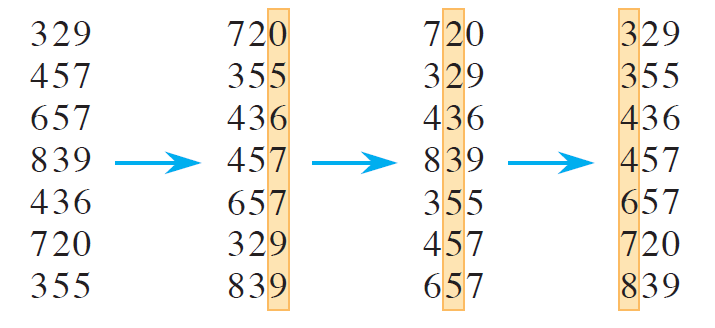
\includegraphics[scale=0.5]{./Immagini/RadixSort.png}
    \caption*{Esempio di ordinamento}
\end{figure}

Radix Sort, per funzionare correttamente, richiede un algoritmo di ordinamento stabile per l'ordinamento delle singole cifre (o caratteri, a seconda del caso).\bigbreak
\noindent Solitamente, come algoritmo sottostante viene utilizzato Counting Sort, il quale, però, nella sua versione tradizionale non è stabile. Infatti, in presenza di chiavi uguali, Counting Sort potrebbe modificare l'ordine relativo degli elementi rispetto all'array di input.\bigbreak
\noindent Per garantire la stabilità, è sufficiente iterare l'array di input in ordine inverso durante la fase di costruzione dell'array di output. In questo modo, quando più elementi hanno la stessa chiave, essi verranno copiati nell'output nell'ordine in cui compaiono nell'input, preservando così la stabilità dell'ordinamento.



\subsubsection{Analisi delle complessità}
\textbf{Caso medio}\quad Considerando \textit{n} elementi da ordinare, ciascuno composto da \textit{d} cifre, e assumendo che ogni cifra possa assumere al più \textit{k} valori distinti, Radix Sort ha una complessità asintotica pari a $\Theta(d(n + k))$.\bigbreak
\noindent Tuttavia, ciò è valido solo se l'algoritmo utilizzato per ordinare le singole cifre (come Counting Sort) ha complessità $\Theta(n + k)$, ovvero è lineare rispetto al numero di elementi e all'ampiezza del dominio delle cifre.\bigbreak
\noindent \textbf{Caso ottimo}\quad Le condizioni del caso ottimo di RadixSort sono:
\begin{itemize}
    \item \textit{d} piccolo;
    \item $k < n$.
\end{itemize}
La complessità rimane $\Theta(d(n + k))$, tuttavia, con valori di $d$ e $k$ costanti si ottiene un $\Theta(n)$.\bigbreak
\noindent \textbf{Caso pessimo}\quad Il caso peggiore si verifica nelle condizioni di:
\begin{itemize}
    \item $d$ elevato (numeri molto grandi);
    \item $k \geq n$ (rende CountingSort inefficiente).
\end{itemize}
La complessità resta $\mathcal{O}(d(n + k))$, ma può degenerare fino a diventare $\mathcal{O}(n\cdot log(n))$
\subsubsection{Motivazioni della scelta}
É stato scelto RadixSort come quarto algoritmo a scelta per il suo approccio innovativo e diverso rispetto agli altri algoritmi selezionati, offrendo una prospettiva di confronto interessante.

\subsubsection{Codice}
\begin{lstlisting}[style=mycodestyle, language=Python]
def RadixSort(arr):
    radix_array = [[], [], [], [], [], [], [], [], [], []]  # array delle cifre
    max_val = max(arr)  # assegno il valore massimo dell'array
    exp = 1 

    while (max_val // exp) > 0:
        while len(arr) > 0:
            val = arr.pop()
            radix_index = (val // exp) % 10
            radix_array[radix_index].append(val)

        for bucket in radix_array:
            while len(bucket) > 0:
                val = bucket.pop()
                arr.append(val)

        exp *= 10
\end{lstlisting}

\section{Misurazioni}

\begin{table} [H]
    \centering
    \begin{tabular}{|c||c|c|c|c|}
        \hline
        & \textbf{QuickSort} & \textbf{QuickSort3Way} & \textbf{CountingSort} & \textbf{RadixSort}\\ [0.1 cm]
        \hline
        \textit{n} & sas & sas & sas & sas\\
        \hline
        \textit{t(n)} & N/A & N/A & N/A & N/A\\
        \hline
    \end{tabular}
\end{table}

\subsection{Analisi delle Prestazioni al Variare della Dimensione dell'Array (Scala Lineare)}
\begin{figure}[H]
    \centering
    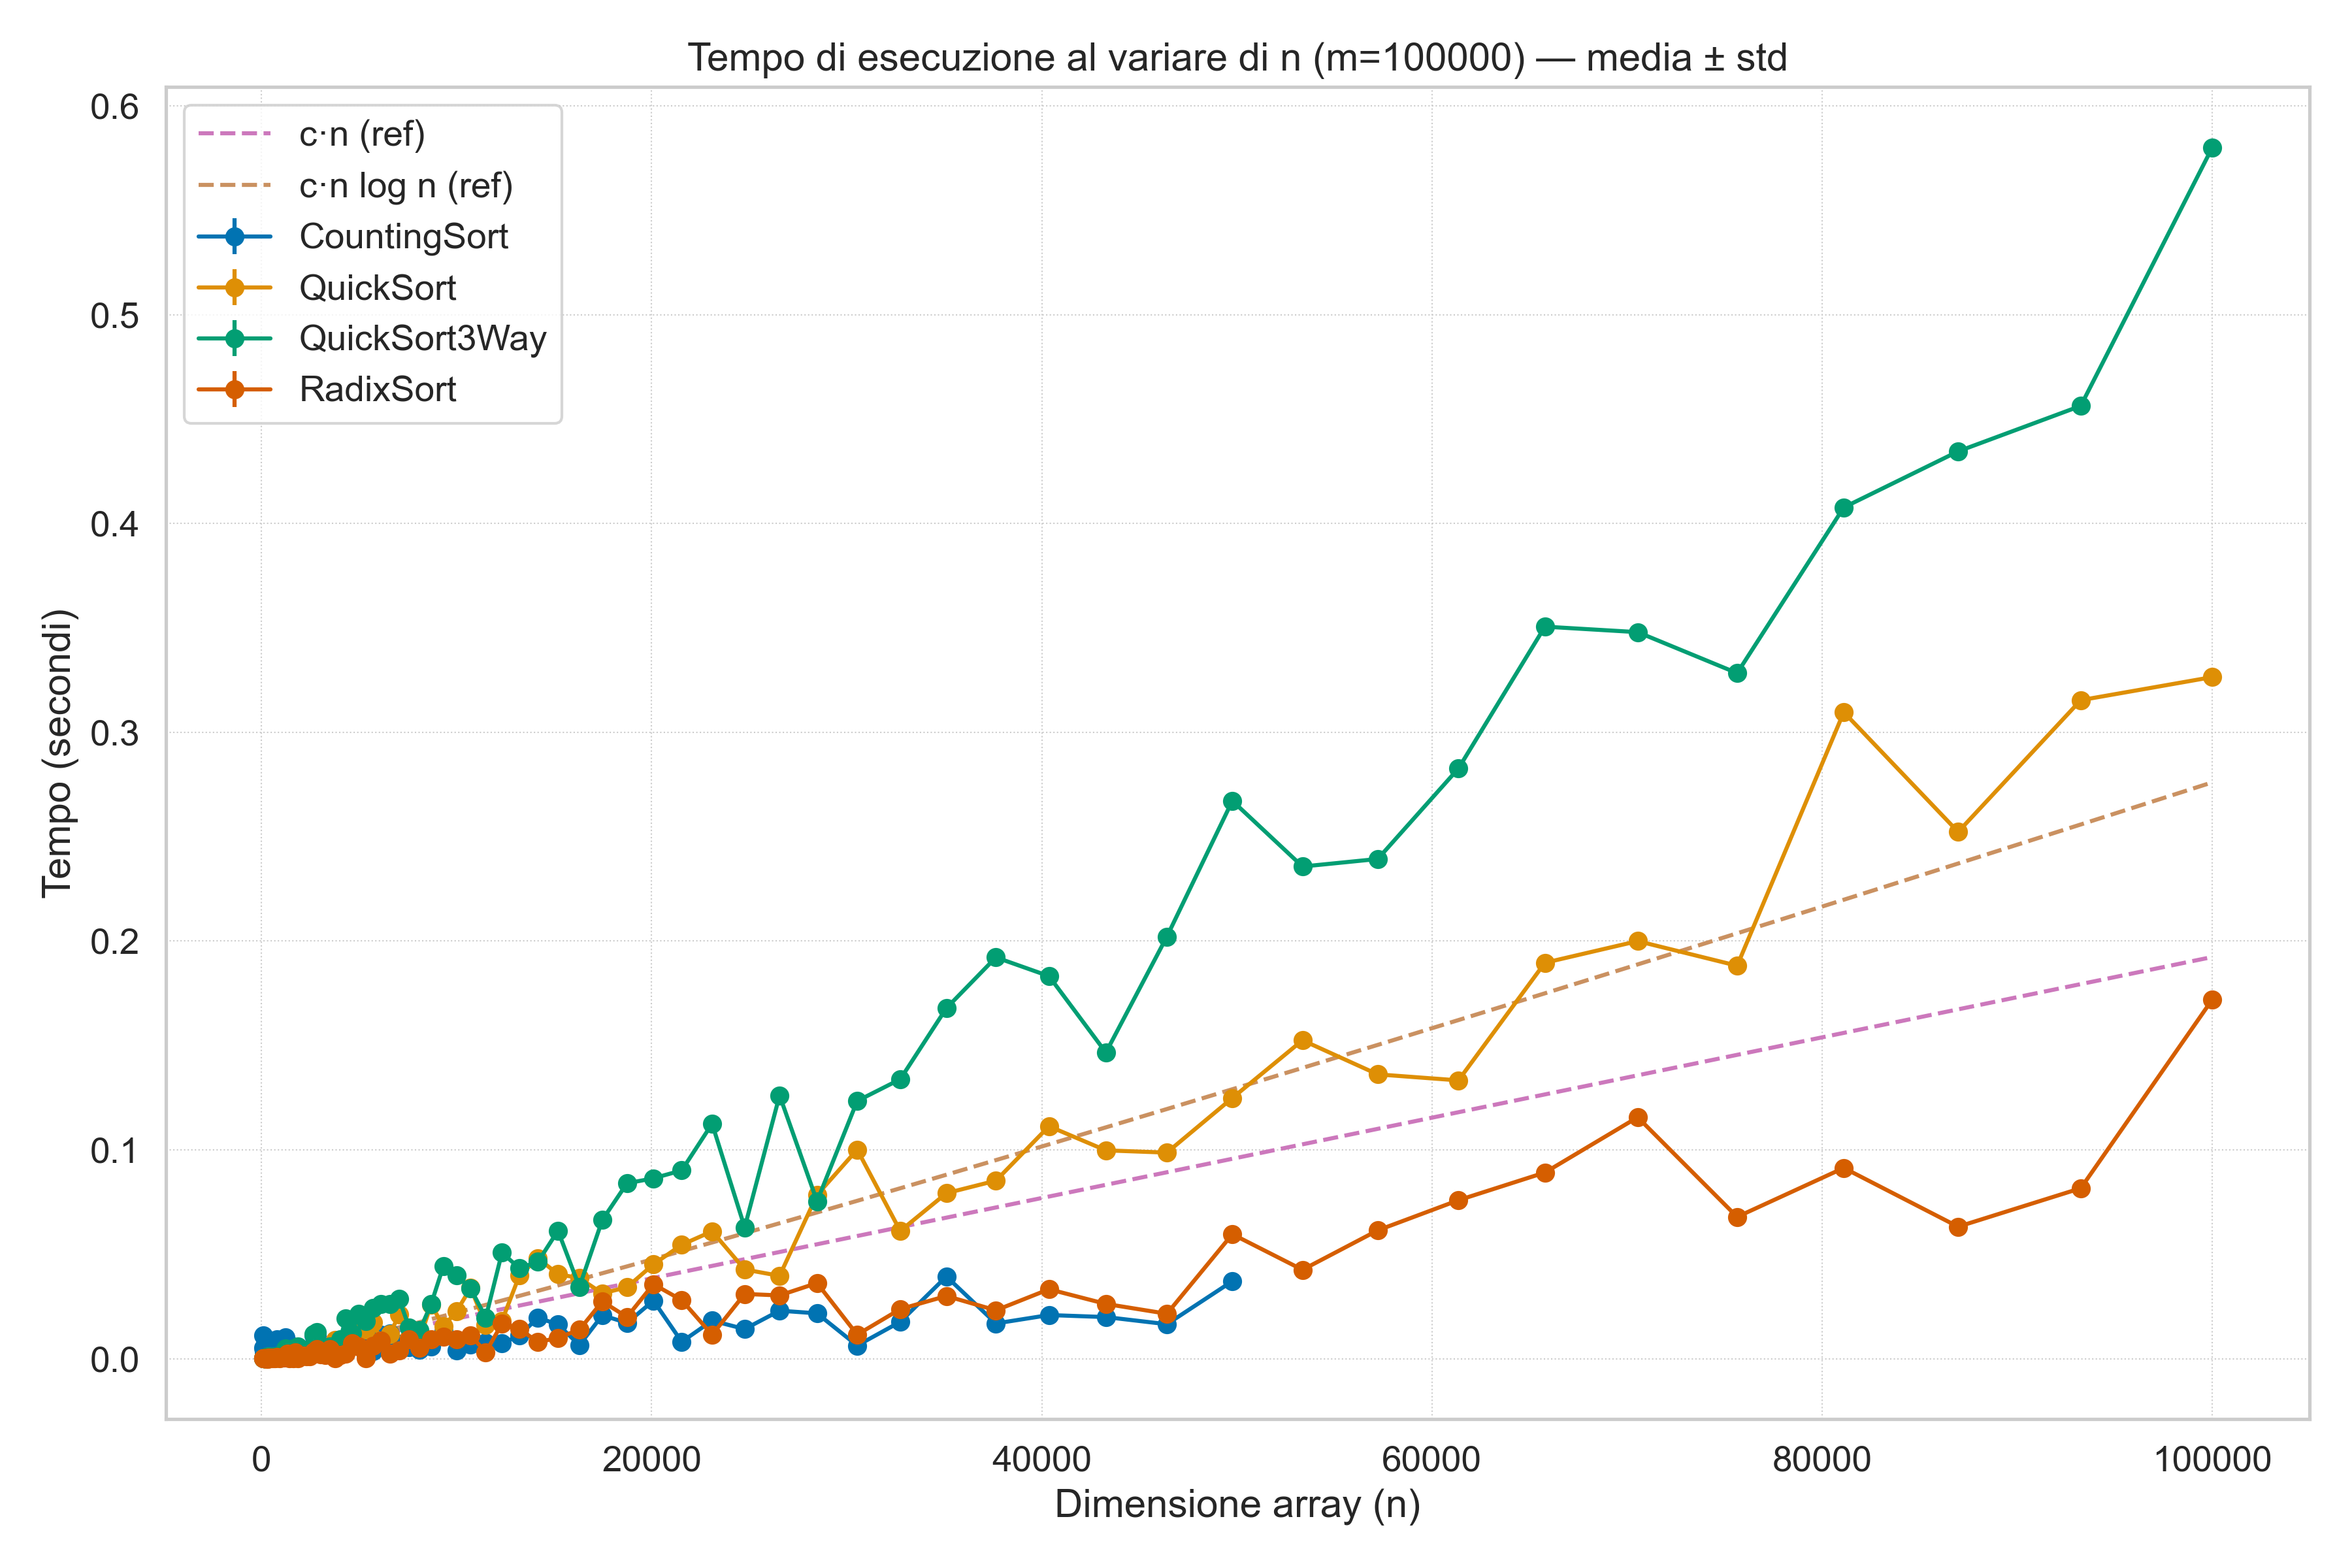
\includegraphics[width=\textwidth]{progetto_ASD__/Relazione/Immagini/tempo_vs_n_lineare_improved.png}
    \caption {\textbf{Tempo vs \(n\) (scala lineare).} Tempo medio di esecuzione al variare di \(n\) (con \(m=100\,000\)). Punti: medie su \(k\) run; barre: deviazione standard. Linee tratteggiate: curve teoriche di riferimento normalizzate su \(n_0\) per confronto pratico.}
    \label{fig:grafico}
\end{figure}

\paragraph{Descrizione e obiettivo}
Questo grafico mostra il tempo medio di esecuzione in funzione della dimensione dell'input \(n\) con \(m\) fissato a 100\,000. Lo scopo è confrontare i tempi assoluti rilevati e visualizzare l'overhead pratico degli algoritmi.

\paragraph{Osservazioni chiave}
\begin{itemize}
  \item I valori assoluti del tempo evidenziano chiaramente le differenze pratiche: algoritmi con complessità asintotica più favorevole (es. \(O(n\log n)\)) si collocano su tempi nettamente inferiori rispetto ad algoritmi quadratici per \(n\) sufficientemente grandi.
  \item Le curve teoriche di riferimento (linee tratteggiate) per \(c\cdot n\) e \(c\cdot n\log n\) sono state normalizzate su un punto di riferimento \(n_0\) ed evidenziano che, sebbene due algoritmi possano avere lo stesso ordine asintotico, le costanti fanno la differenza nelle dimensioni realistiche dell'esperimento.
  \item Le barre di deviazione standard, se contenute, confermano la ripetibilità sperimentale; eventuali picchi o rumore debbono essere commentati (carico di sistema, garbage collection, variazioni nella generazione degli input).
\end{itemize}

\paragraph{Caveat interpretativi}
Non trarre conclusioni sull'ordine di crescita esclusivamente osservando la curvatura in scala lineare: curve asintoticamente diverse possono essere vicine nei range sperimentali limitati. Per questo motivo è utile affiancare il grafico con la versione log-log (Grafico~2).

\subsection{Analisi delle Prestazioni al Variare della Dimensione dell'Array (Scala Log-Log)}
\begin{figure}[H]
\centering
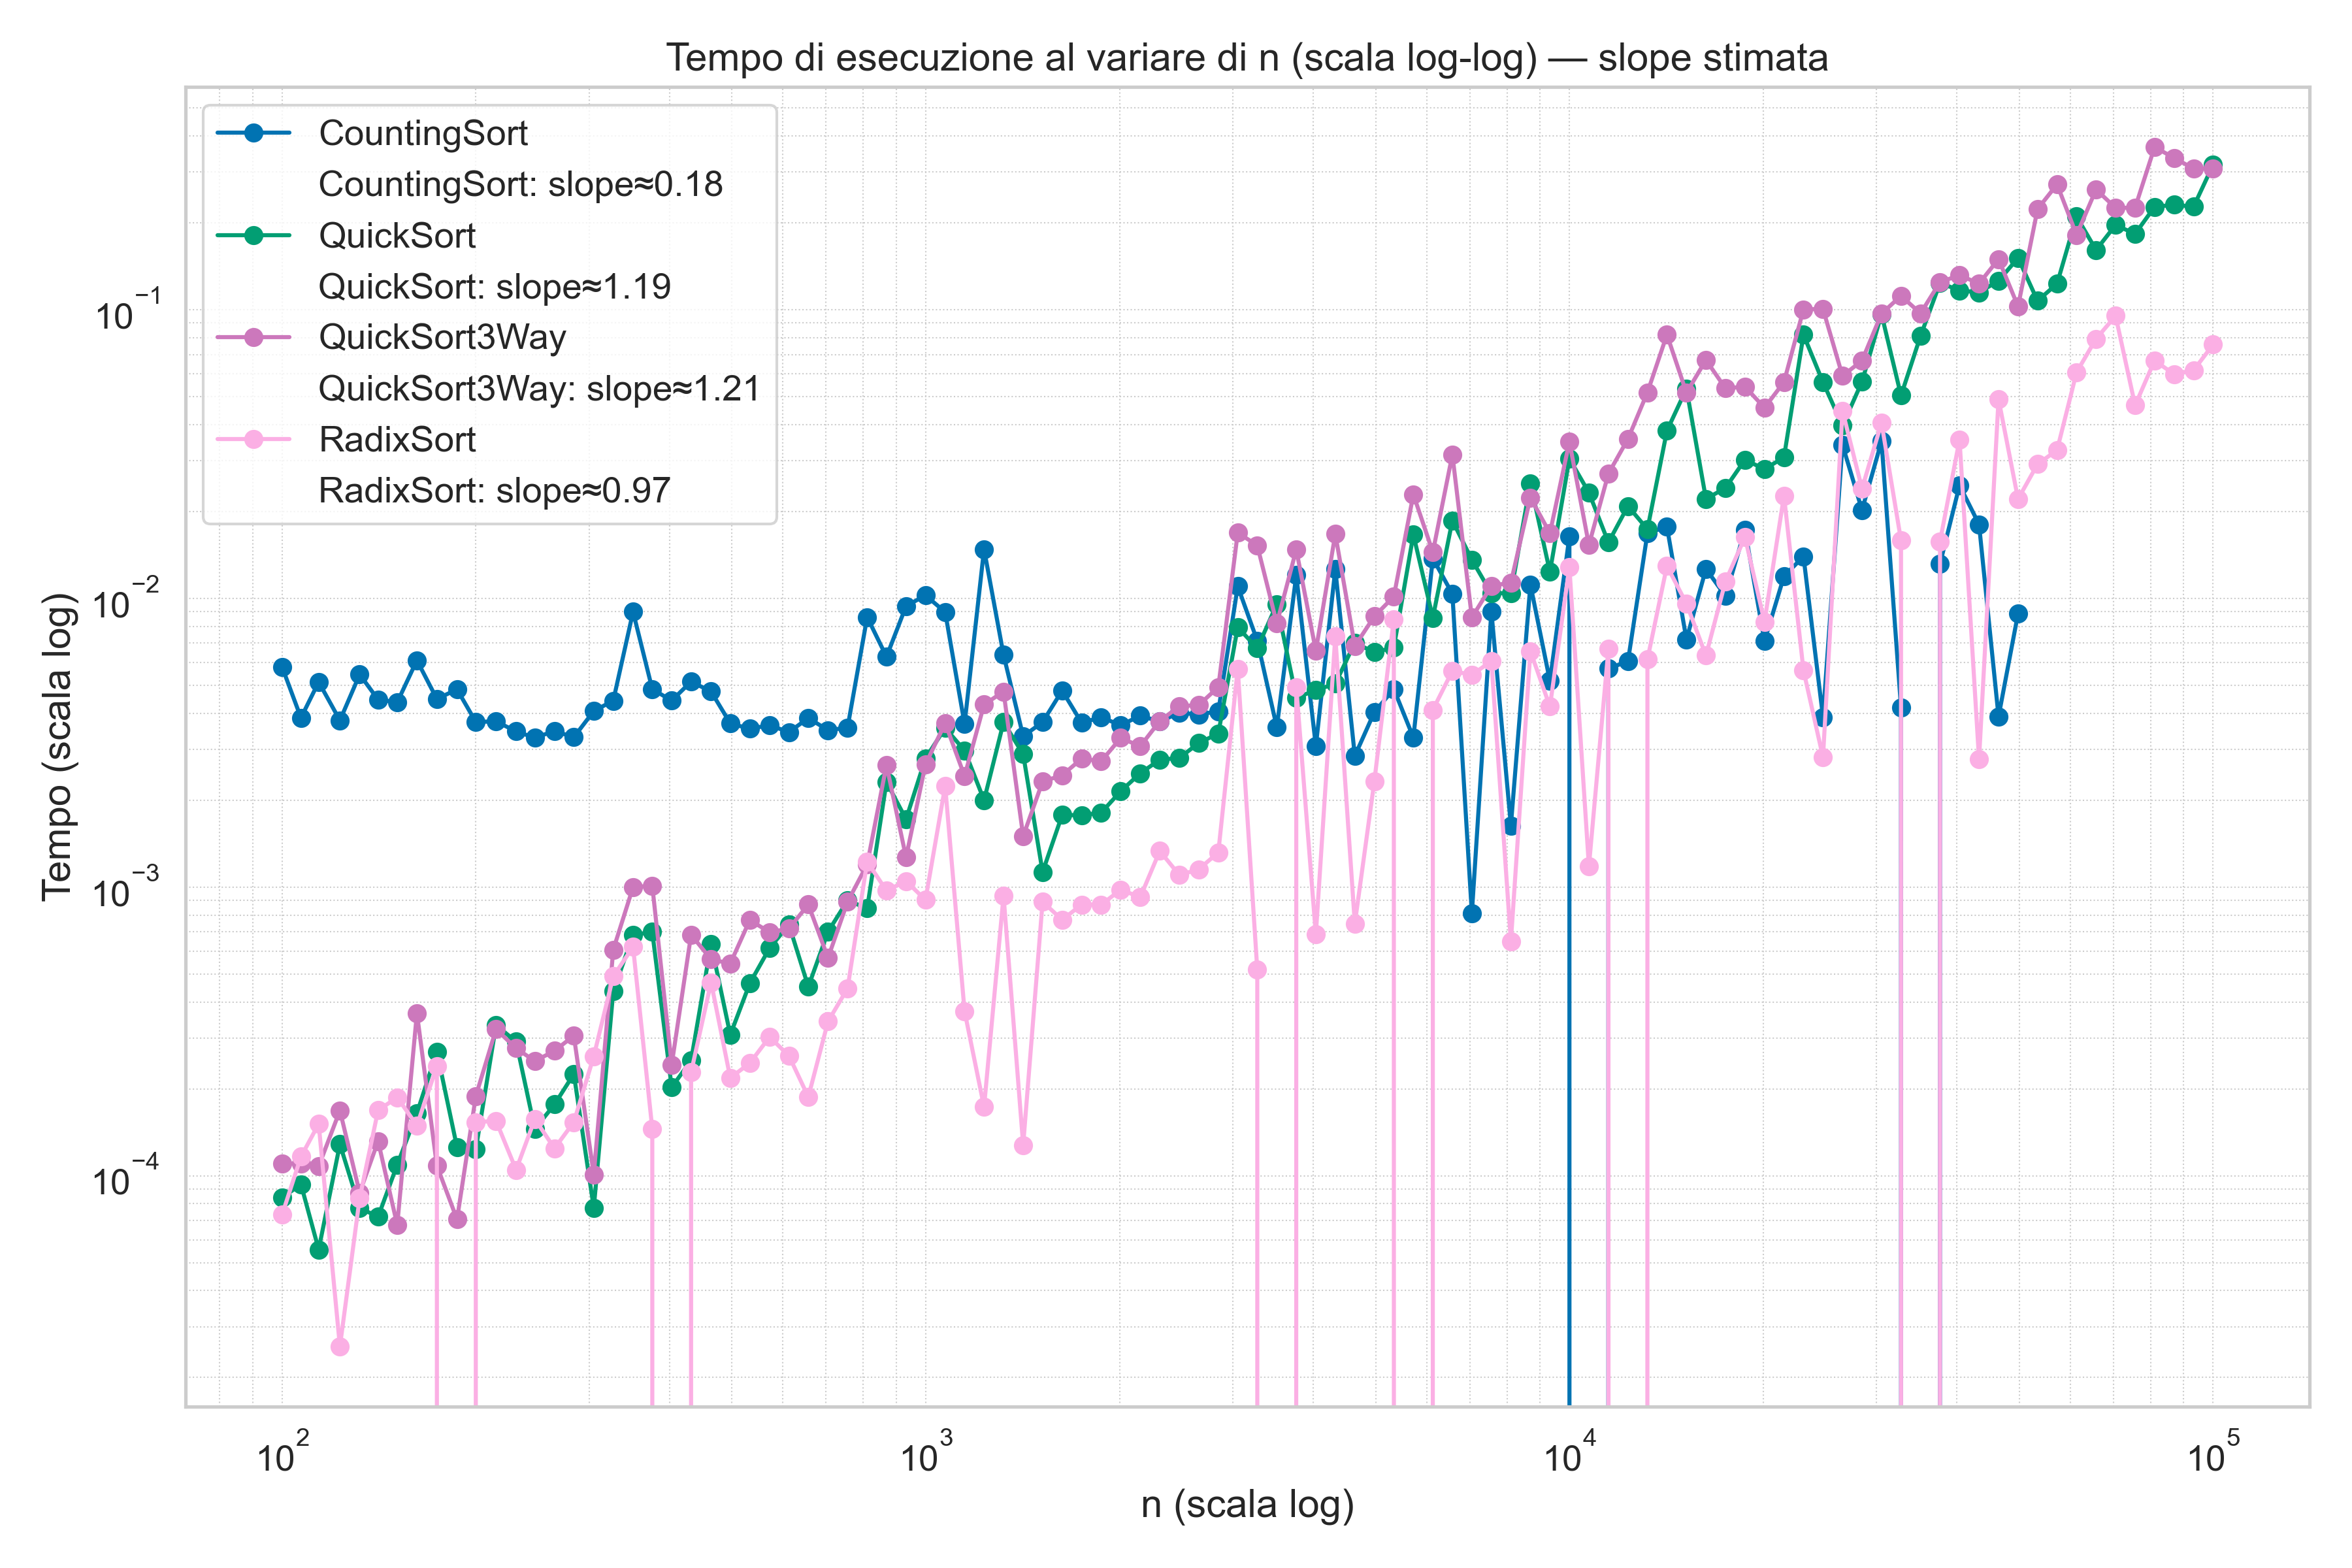
\includegraphics[width=0.9\textwidth]{progetto_ASD__/Relazione/Immagini/tempo_vs_n_loglog_improved.png}
\caption{\textbf{Tempo vs \(n\) (scala log-log).} Regressione lineare su \(\log\)-\(\log\) per stimare la pendenza empirica \(a\) tale che \(\text{time}\approx C n^{a}\). Valori di pendenza stimati riportati in legenda. Nota: per complessità \(O(n\log n)\) la pendenza reale tende a 1.}
\label{fig:variazione_m}
\end{figure}

\paragraph{Descrizione e obiettivo}
La scala log-log è utilizzata per stimare la relazione di tipo potenza tra tempo e dimensione dell'input: una regressione lineare tra \(\log(\text{time})\) e \(\log(n)\) fornisce una stima empirica dell'esponente effettivo.

\paragraph{Interpretazione della pendenza}
\begin{itemize}
  \item Se la regressione restituisce una pendenza \(a\) tale che \(\log(\text{time}) \approx a\log n + b\), allora \(\text{time} \approx C\cdot n^{a}\).
  \item Per complessità \(O(n\log n)\) la pendenza \(a\) tende a 1 per \(n\) grandi (poiché \(\log n\) cresce lentamente rispetto a potenze), dunque una pendenza empirica leggermente maggiore di 1 è coerente con \(n\log n\) su intervalli finiti; non implica automaticamente un ordine polinomiale effettivo con esponente \(>1\).
  \item Una pendenza prossima a 2 corrisponderebbe a comportamento quadratico \(O(n^2)\).
\end{itemize}

\subsection{Impatto del Range dei Valori sulle Prestazioni (Scala Lineare)}
\begin{figure}[H]
\centering
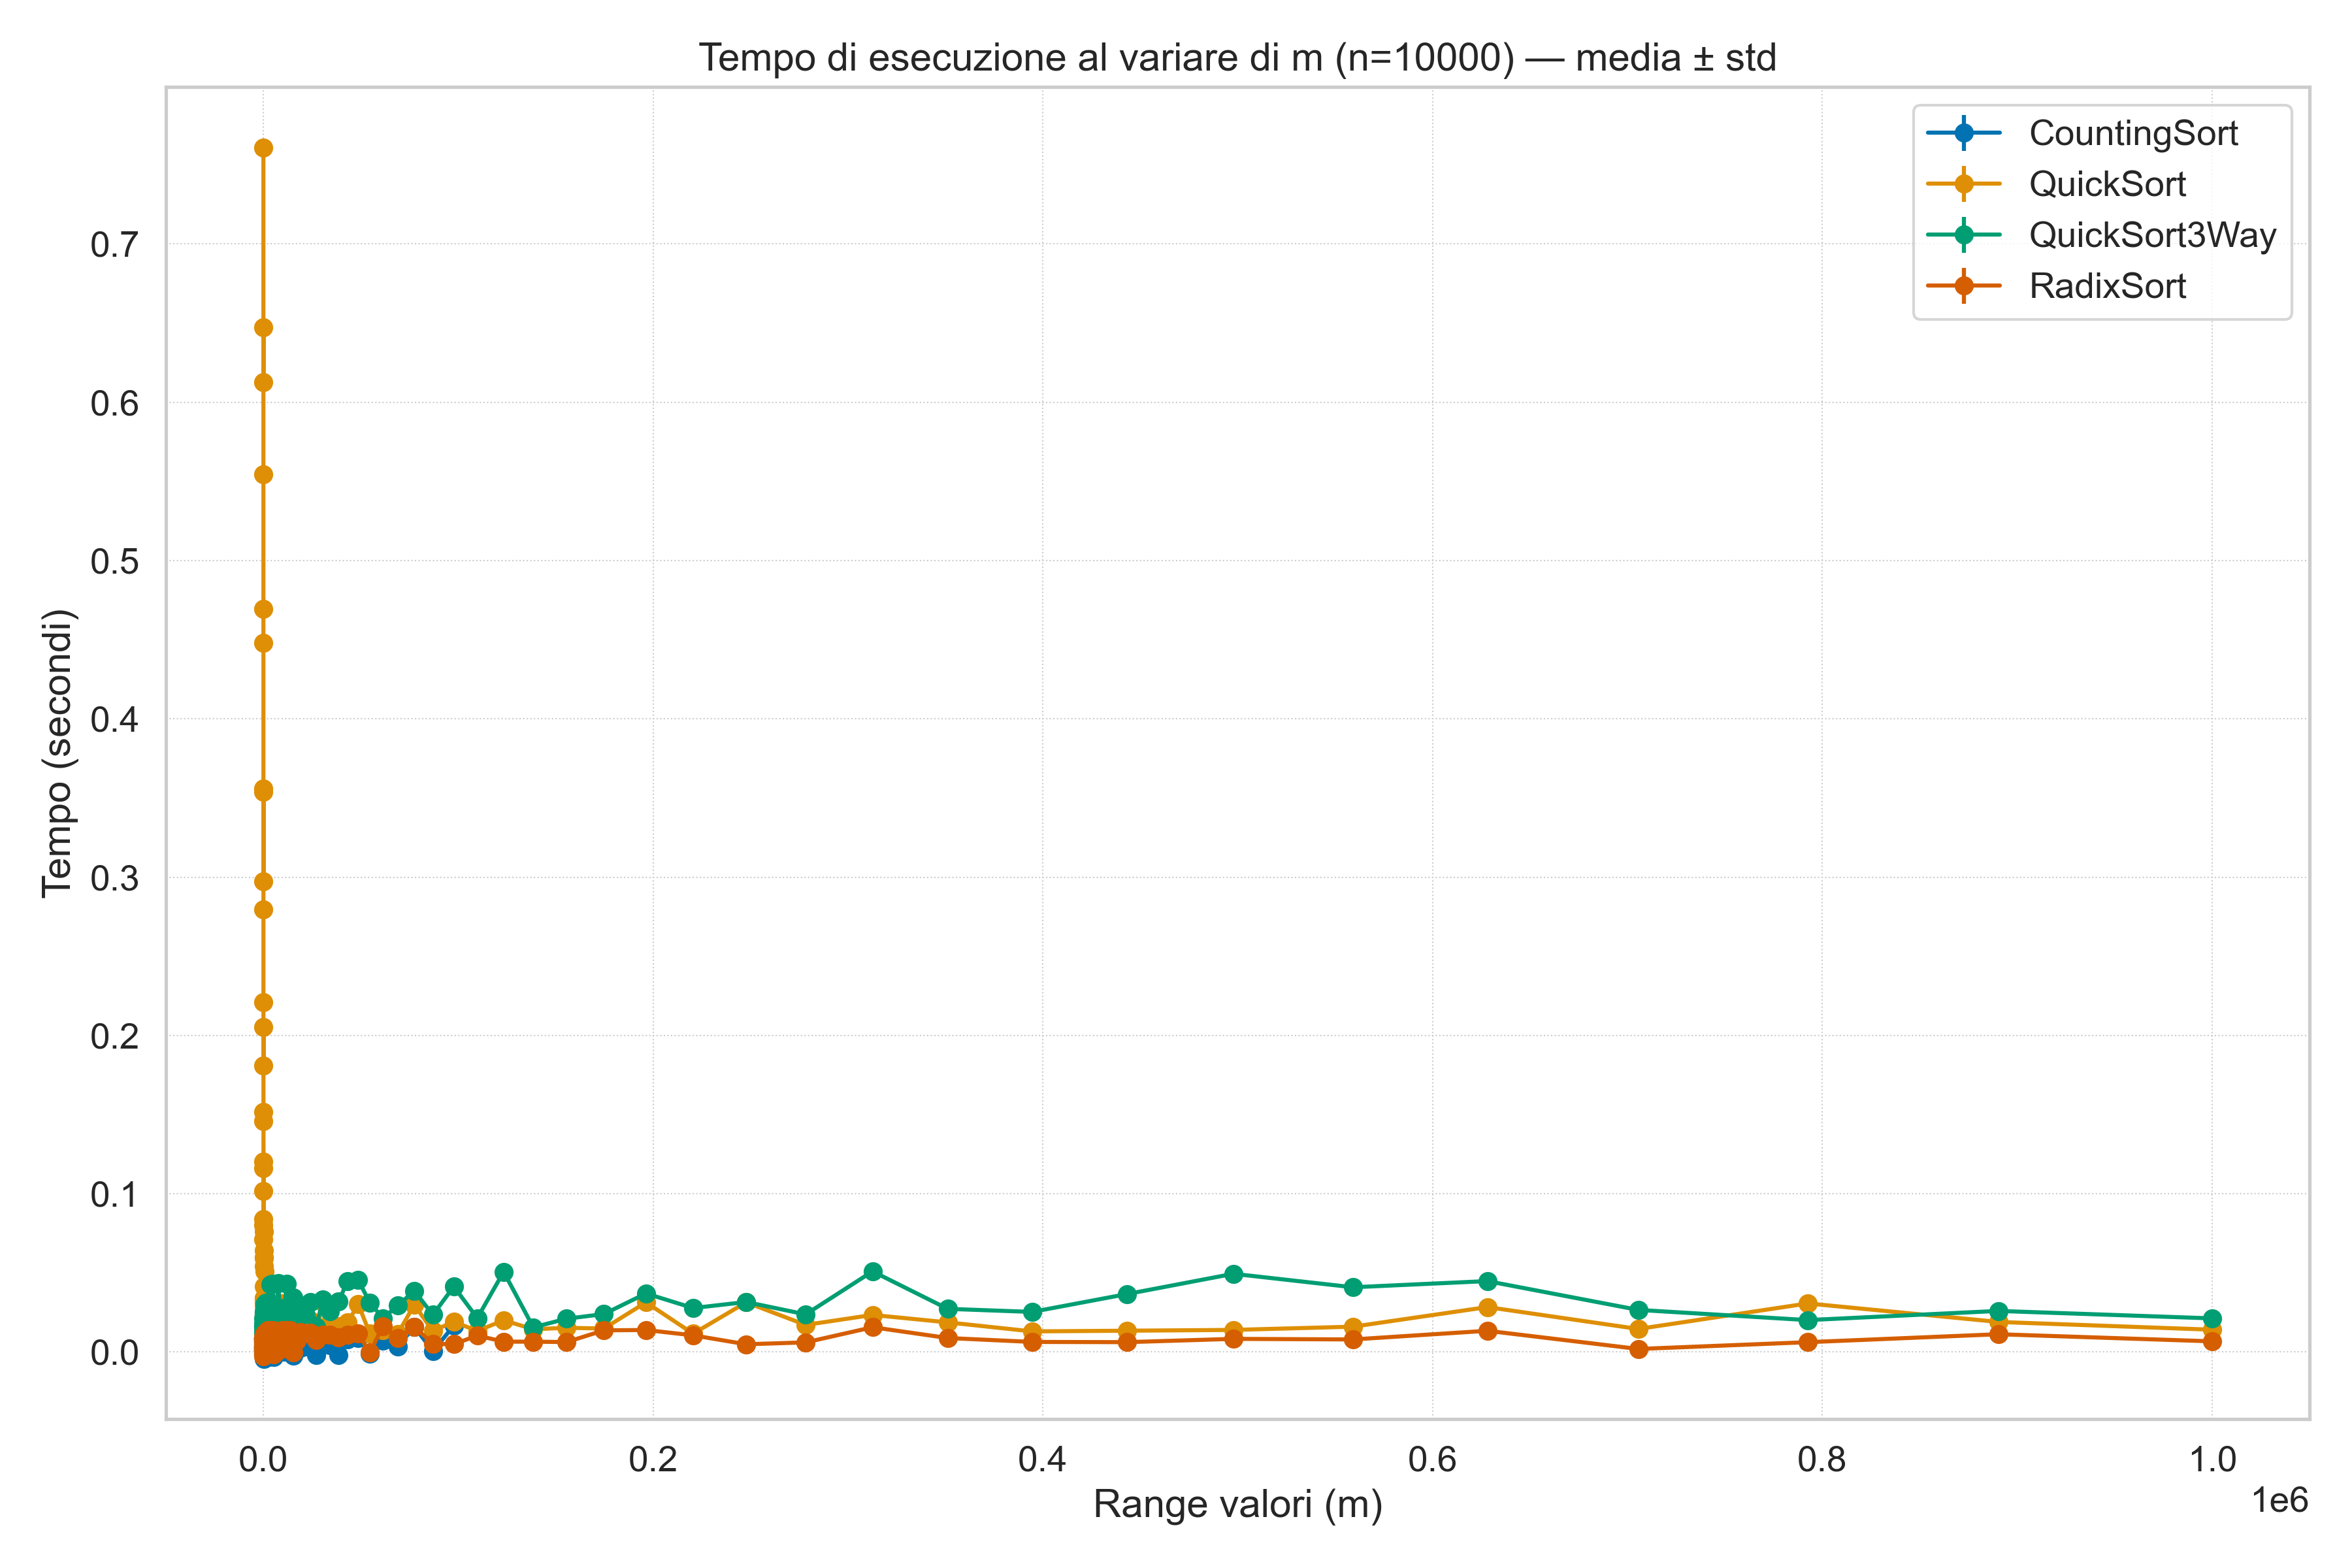
\includegraphics[width=0.9\textwidth]{progetto_ASD__/Relazione/Immagini/tempo_vs_m_lineare_improved.png}
\caption{\textbf{Tempo vs \(m\) (scala lineare).} Effetto del range dei valori \(m\) su algoritmi comparativi e non comparativi (con \(n\) fissato). Barre: deviazione standard. Nota: Counting Sort richiede memoria proporzionale a \(m\).}
\label{fig:variazione_m}
\end{figure}

\paragraph{Descrizione e obiettivo}
Questo grafico valuta l'impatto del range dei valori \(m\) (es. dominio dei numeri generati) sul tempo degli algoritmi, con \(n\) fissato. È particolarmente rilevante per algoritmi non comparativi come Counting Sort.

\paragraph{Osservazioni chiave}
\begin{itemize}
  \item \textbf{Counting Sort:} il tempo cresce sensibilmente con \(m\) a causa dell'allocazione e inizializzazione dell'array dei contatori di dimensione \(m\). Anche se il numero di elementi \(n\) è piccolo, un \(m\) grande comporta costi non trascurabili.
  \item \textbf{Radix Sort:} dipende invece dal numero di cifre \(d\) e dalla base \(b\): per chiavi con rappresentazione a lunghezza fissa e \(d\) costante, Radix può rimanere efficace anche per \(m\) grandi.
  \item Altri algoritmi comparativi (QuickSort, QuickSort 3-way) risultano relativamente insensibili al valore di \(m\) perché la loro complessità dipende principalmente da \(n\).
\end{itemize}

\subsection{Analisi dell'Impatto del Range dei Valori (Scala Log-Log)}
\begin{figure}[H]
\centering
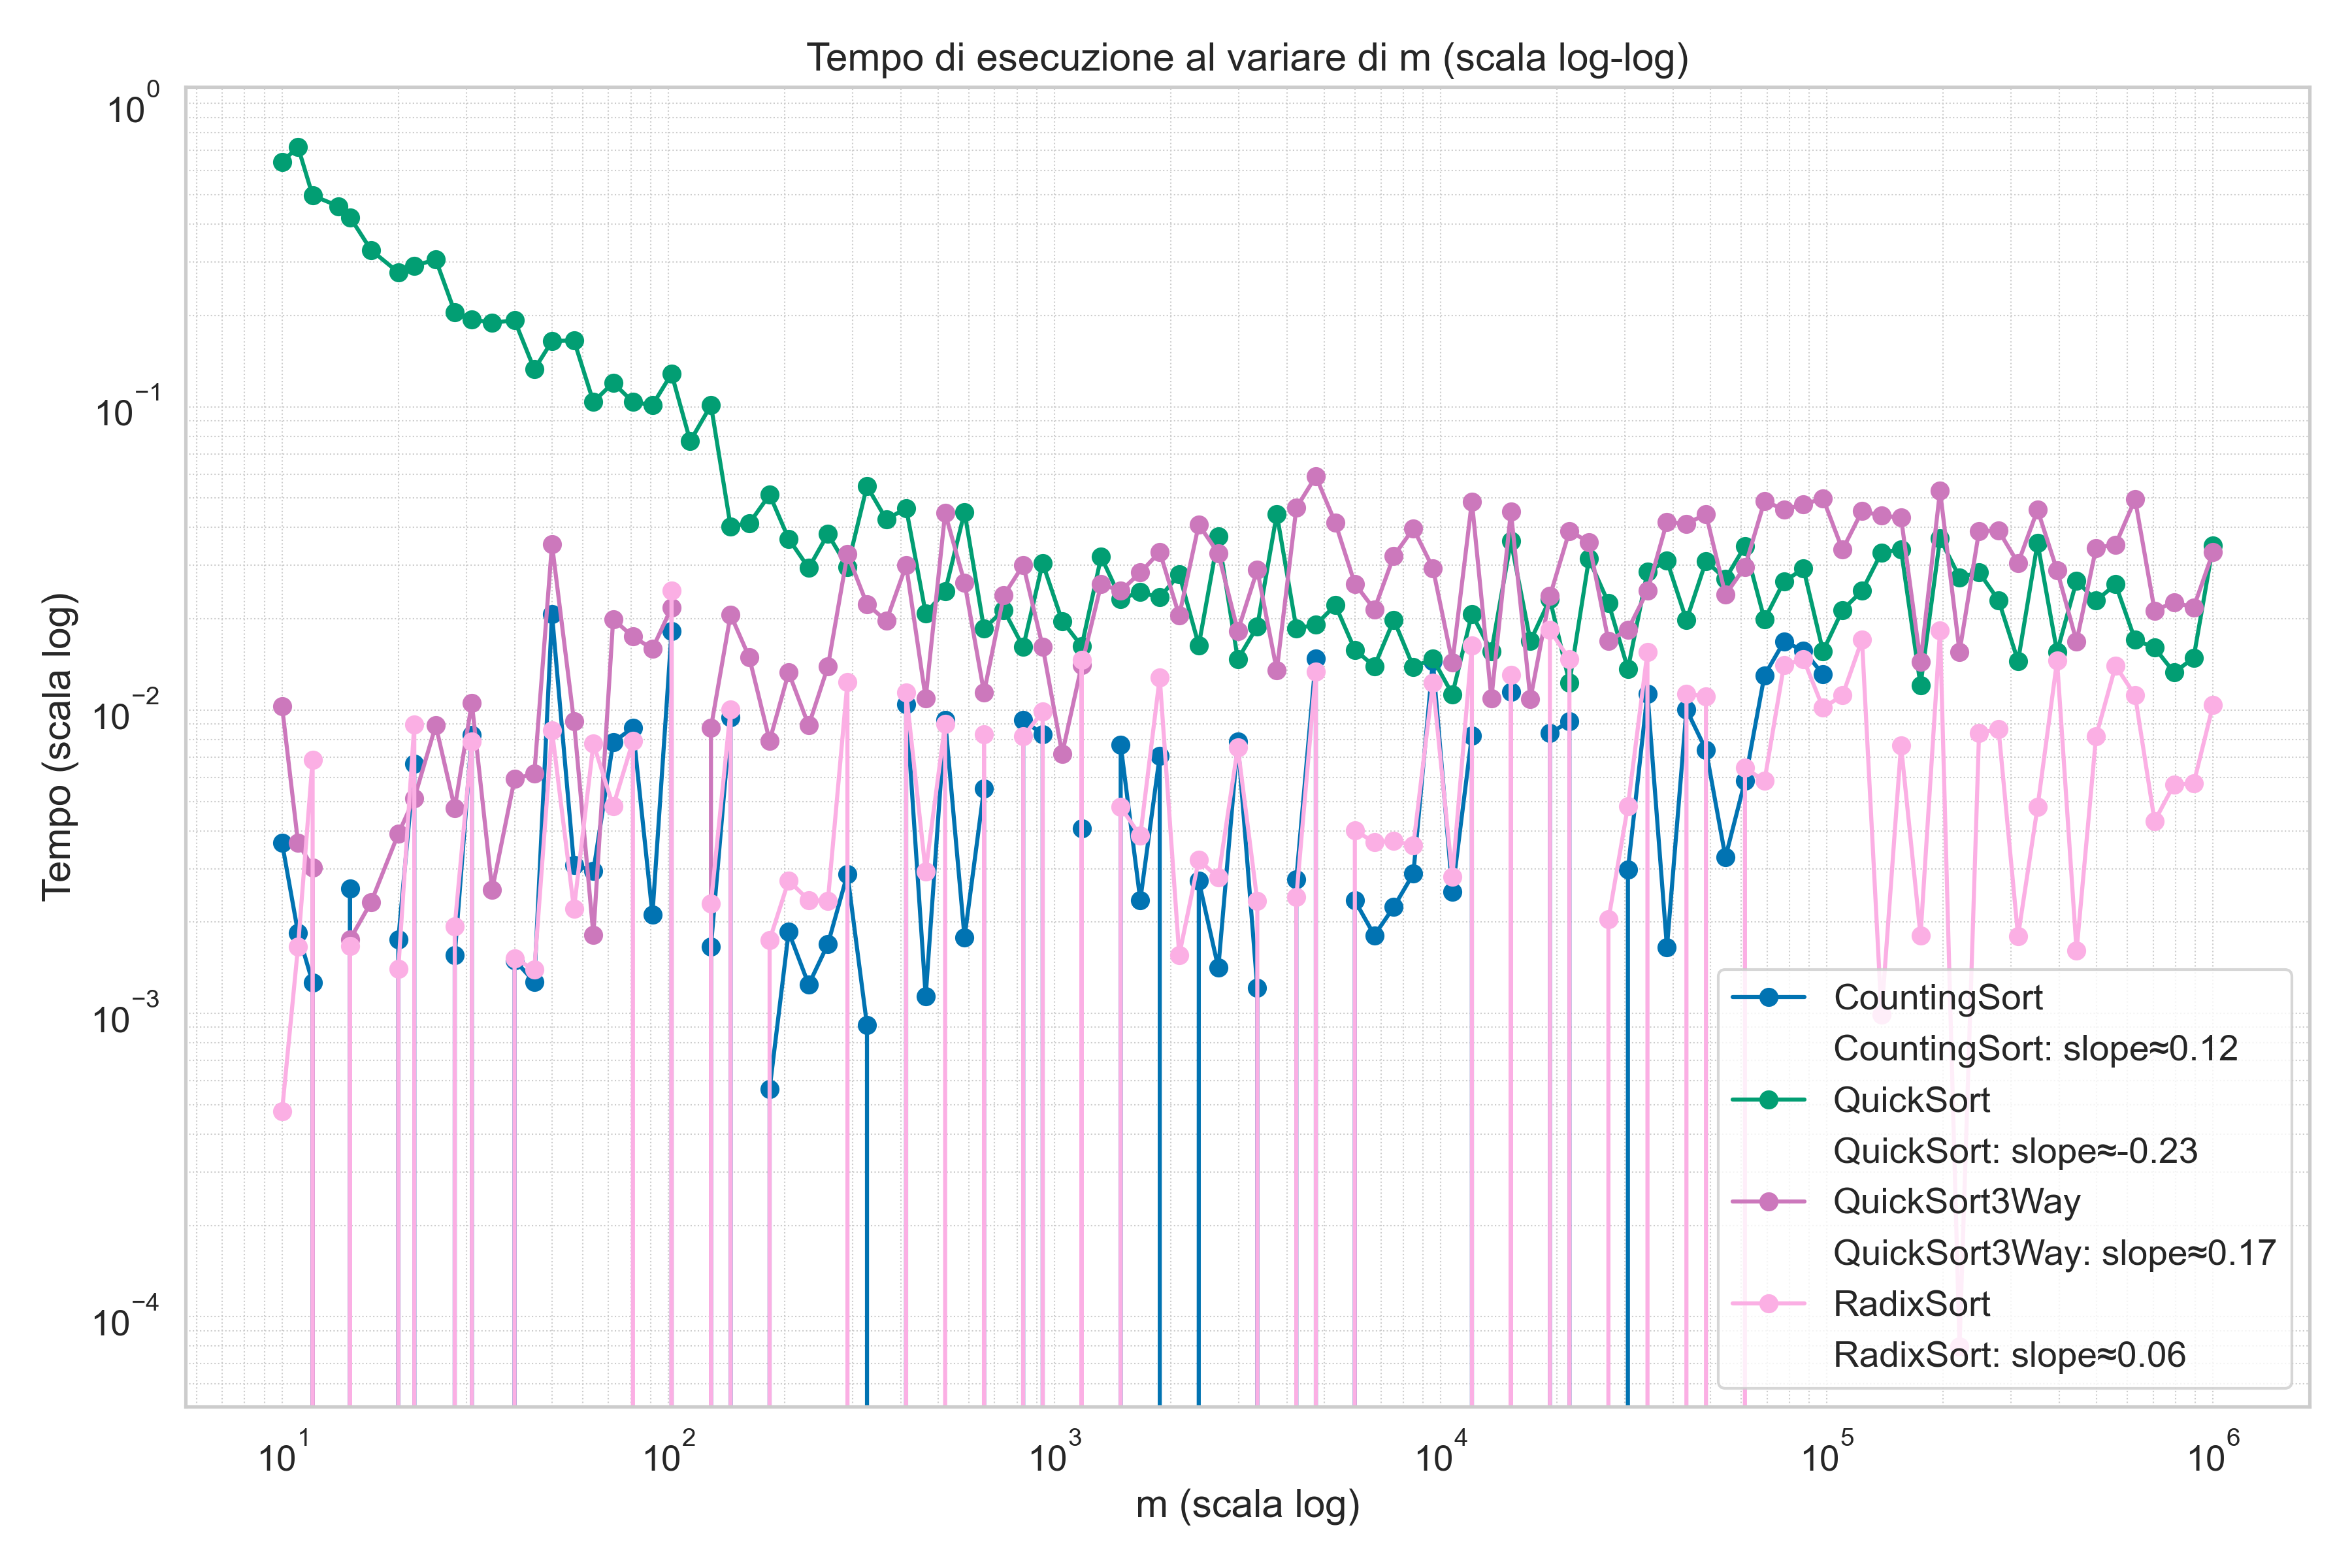
\includegraphics[width=0.9\textwidth]{progetto_ASD__/Relazione/Immagini/tempo_vs_m_loglog_improved.png}
\caption{\textbf{Tempo vs \(m\) (scala log-log).} Regressione log-log per stimare la dipendenza dal range \(m\). Pendenze stimate riportate nella legenda. Counting Sort mostra tipicamente pendenza circa 1 dovuta all'azzeramento dell'array dei contatori.}
\label{fig:variazione_m}
\end{figure}

\paragraph{Descrizione e obiettivo}
Versione log-log del Grafico~3: utile a stimare il comportamento asintotico rispetto a \(m\) (quando ha senso interpretare come potenza).

\paragraph{Interpretazione}
\begin{itemize}
  \item Una pendenza \(a\approx 1\) per Counting Sort indica comportamento lineare rispetto a \(m\) (atteso per certe fasi dell'algoritmo come azzeramento dell'array dei contatori).
  \item Se Radix presenta pendenza molto più bassa o platea, ciò indica che il costo non cresce direttamente con \(m\) ma è legato a parametri diversi (numero di cifre \(d\), base \(b\)).
\end{itemize}

\subsection{Analisi dei Casi Peggiori per gli Algoritmi QuickSort}
\begin{figure}[H]
\centering
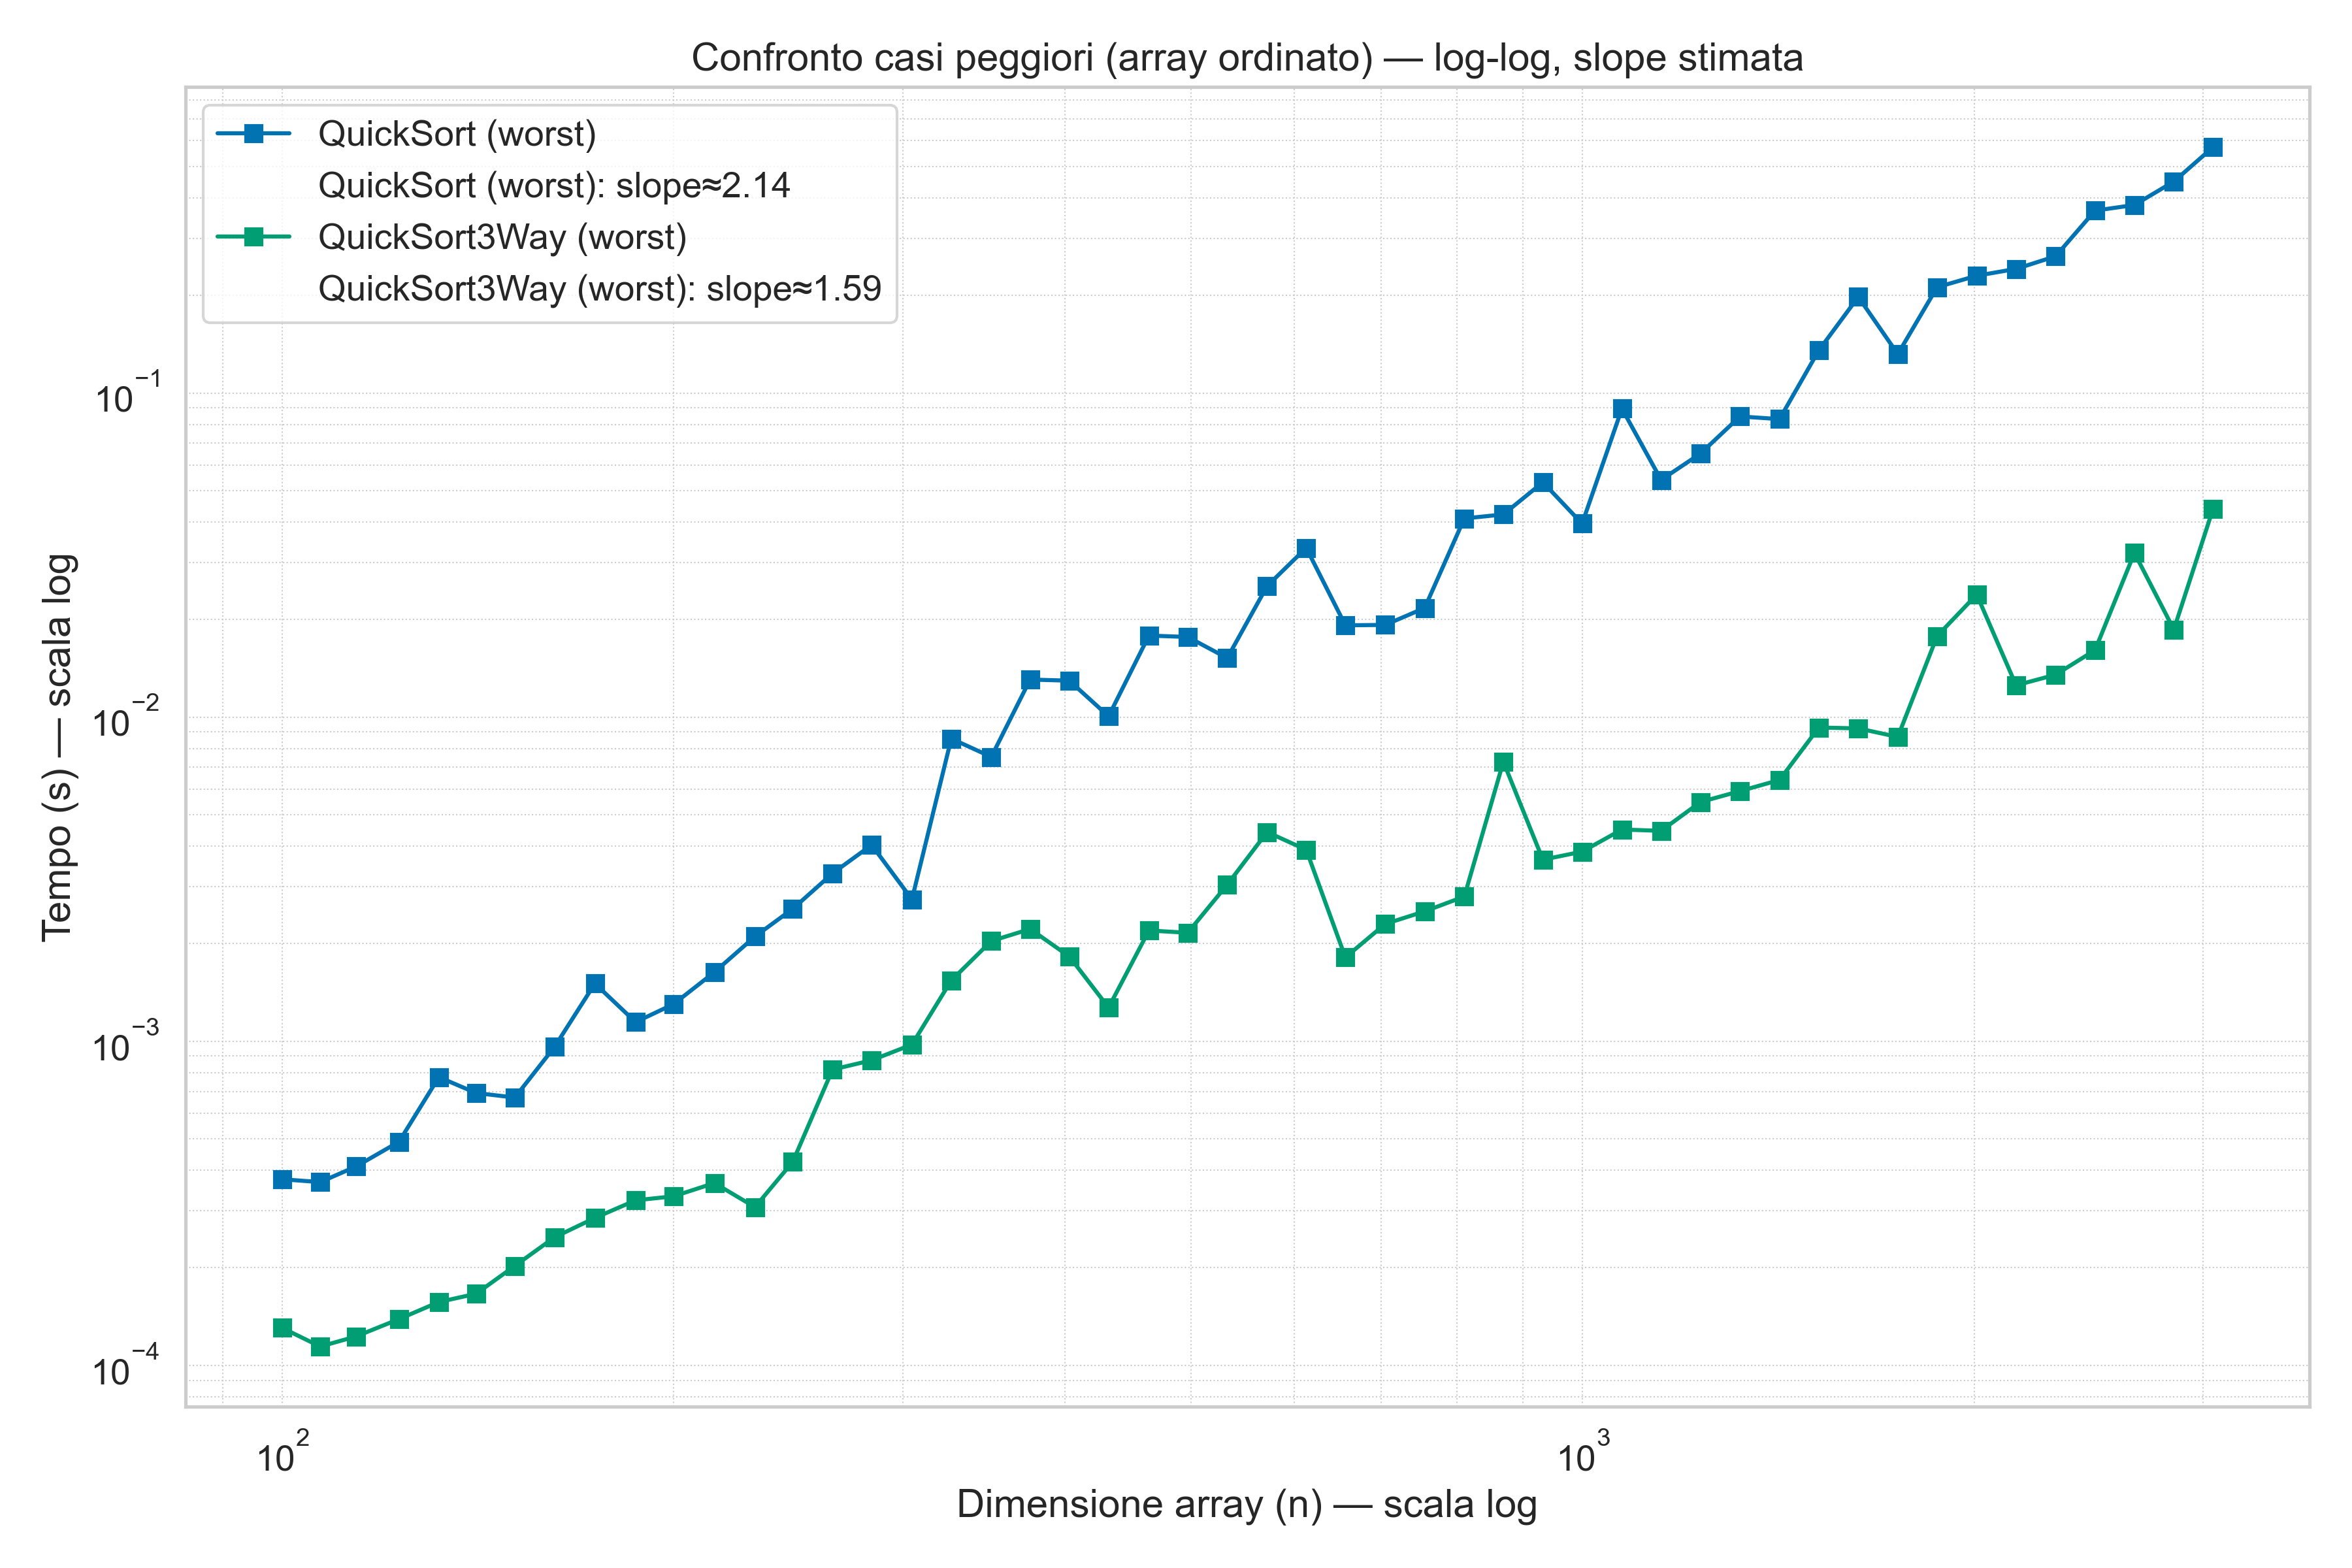
\includegraphics[width=0.9\textwidth]{progetto_ASD__/Relazione/Immagini/confronto_casi_peggiori_loglog.png}
\caption{\textbf{Confronto casi peggiori (log-log).} Prestazioni su input ordinato; regressioni log-log usate per stimare l'esponente empirico. QuickSort classico mostra il peggior comportamento se non protetto da scelte pivot robuste.}
\label{fig:variazione_m}
\end{figure}

\paragraph{Descrizione e obiettivo}
Questo grafico confronta le prestazioni degli algoritmi sul caso avverso (ad esempio array già ordinato), con l'obiettivo di evidenziare degradazioni asintotiche, in particolare del QuickSort classico.

\paragraph{Osservazioni e interpretazioni}
\begin{itemize}
  \item \textbf{QuickSort classico:} il pivot mal scelto può causare la ricorrenza degenerata \(T(n)=T(n-1)+\Theta(n)\) e quindi \(T(n)=\Theta(n^2)\); su log-log ciò si riflette con una pendenza vicino a 2.
  \item \textbf{QuickSort 3-way o pivot randomizzato:} mostrano pendenze più vicine a 1 (o lievemente sopra) anche sullo stesso set di input, a dimostrazione della robustezza della scelta pivot o della tecnica 3-way in presenza di molteplici valori uguali.
\end{itemize}

\subsection{Analisi Comparativa dell'Impatto del Range su Algoritmi Non Comparativi}
\begin{figure}[H]
\centering
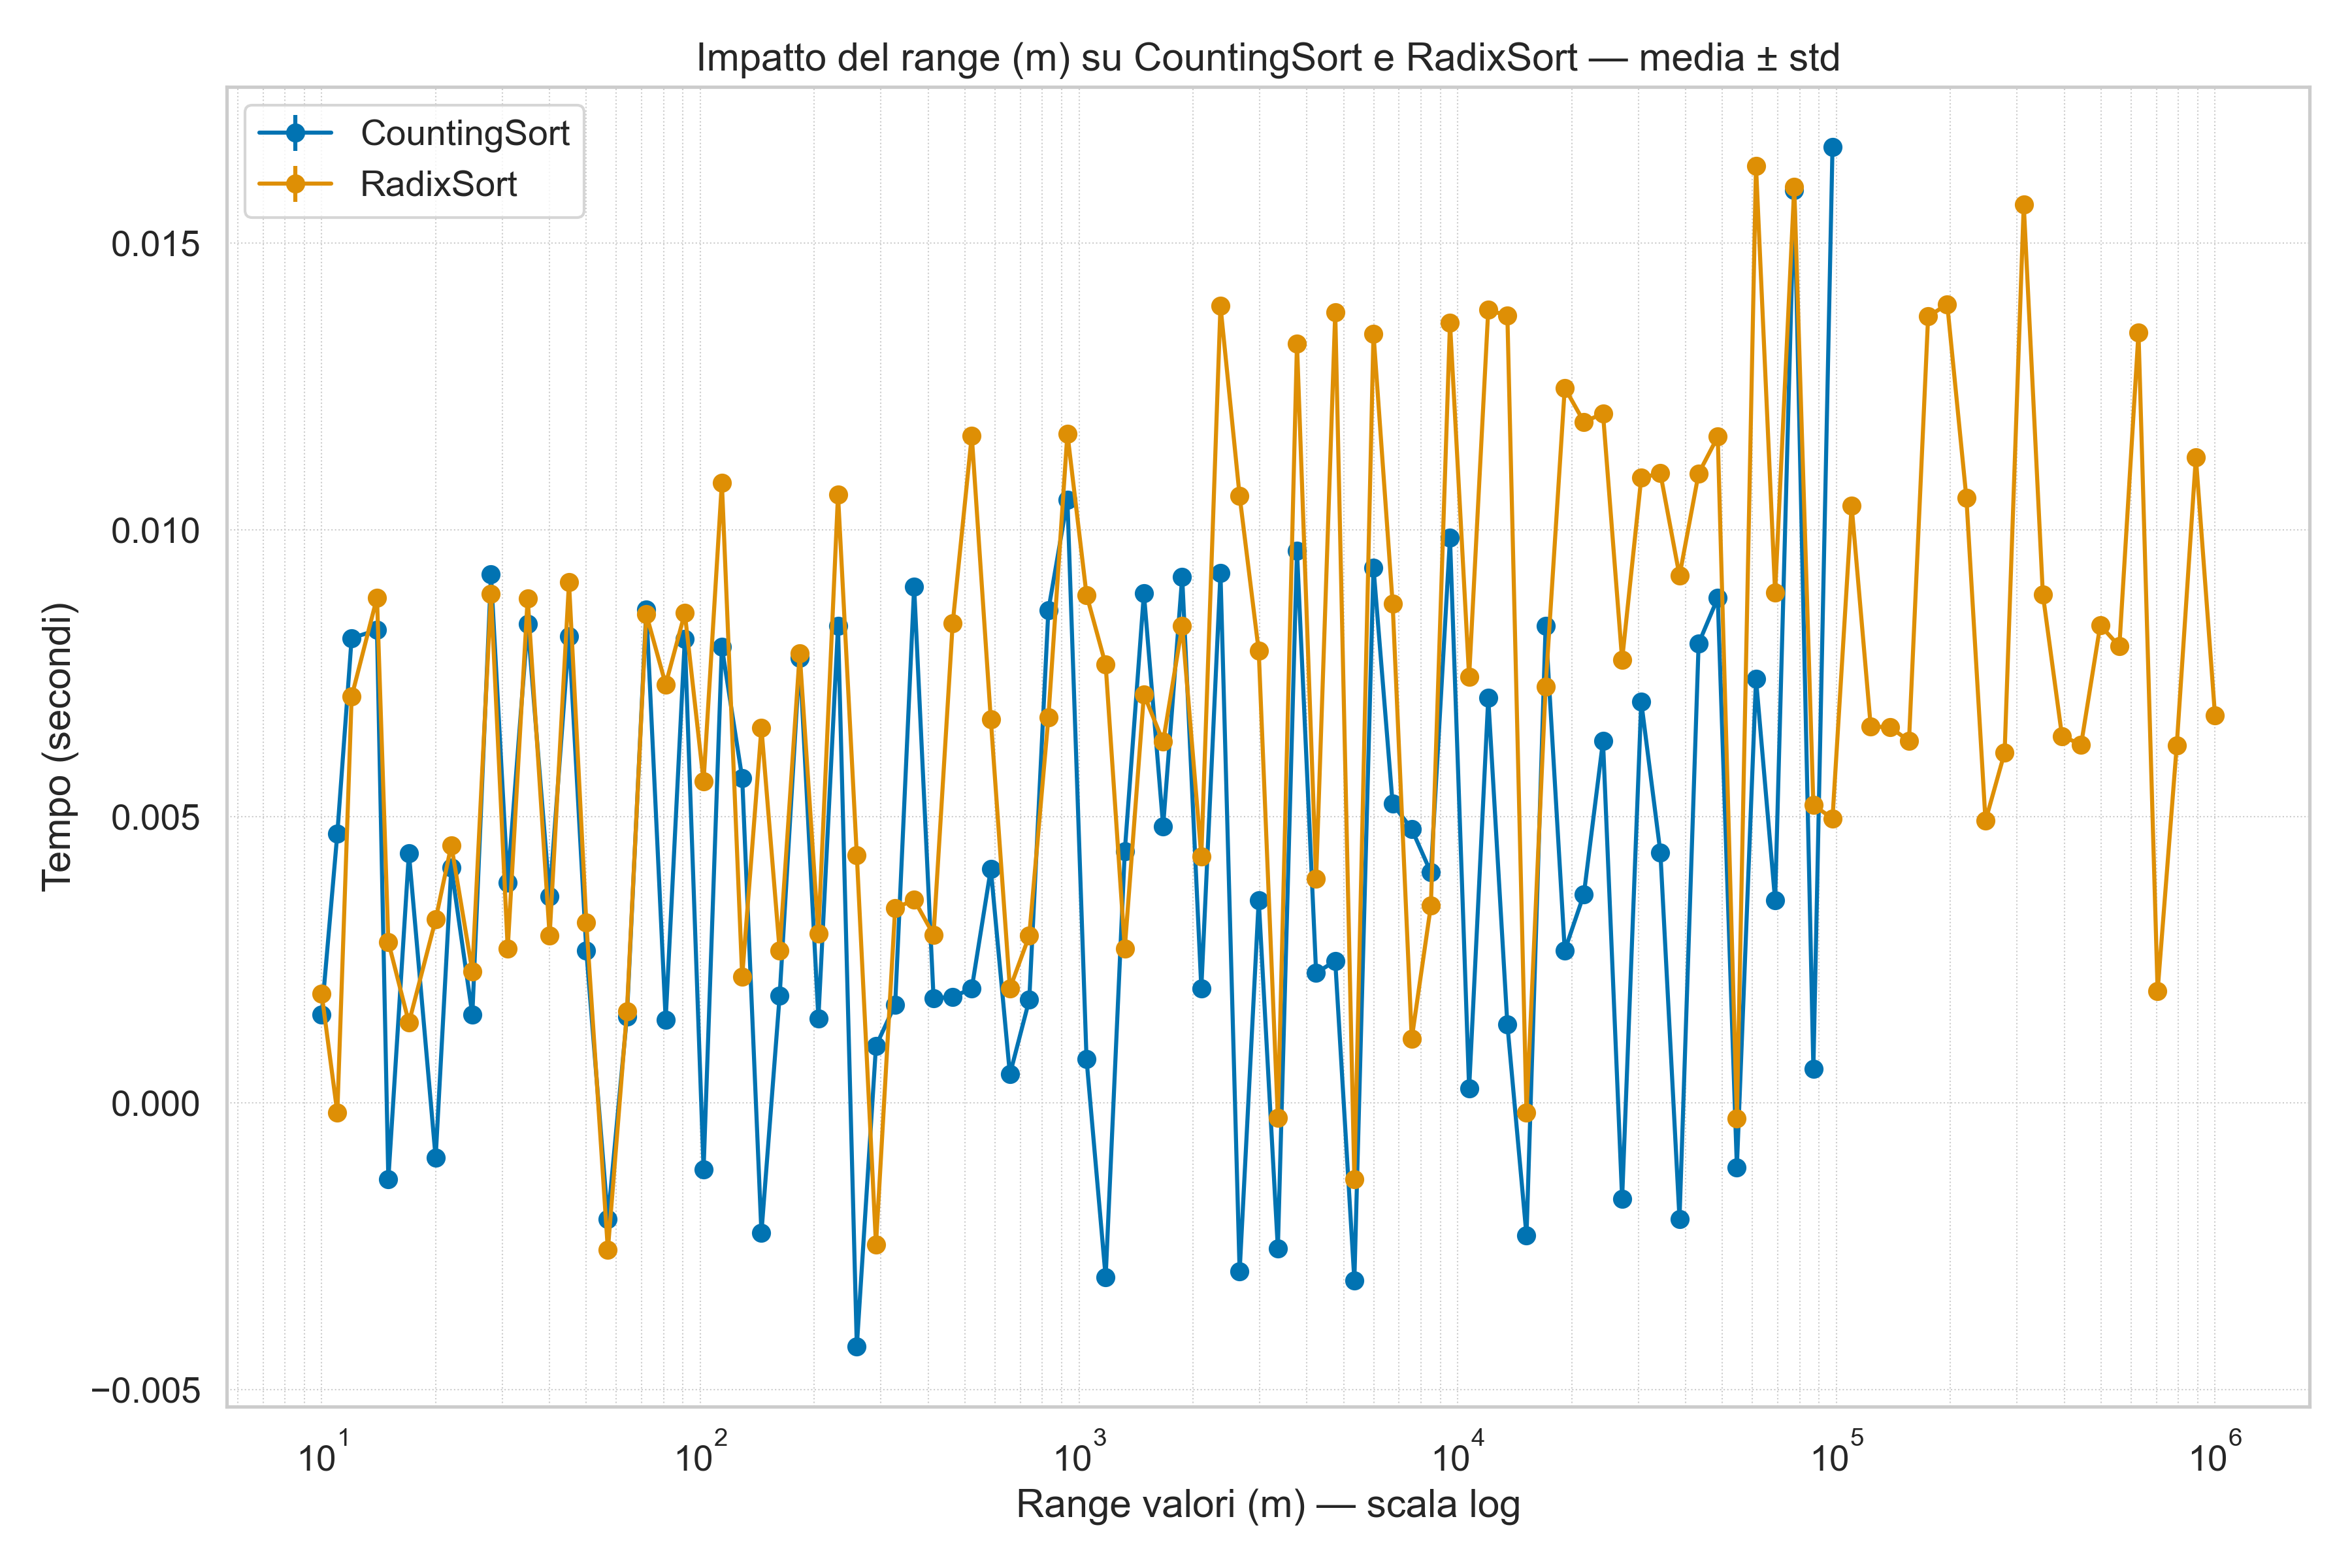
\includegraphics[width=0.9\textwidth]{progetto_ASD__/Relazione/Immagini/impatto_m_counting_radix_improved.png}
\caption{\textbf{Impatto di \(m\) su CountingSort e RadixSort (asse \(m\) logaritmico).} Confronto diretto che mostra il passaggio di regime: Counting Sort è competitivo per \(m\) piccoli, ma diventa inefficiente per \(m\) grandi per motivi di memoria e overhead di inizializzazione. Radix mostra migliore scalabilità nel caso di chiavi con numero di cifre limitato.}
\label{fig:variazione_m}
\end{figure}

\paragraph{Descrizione e obiettivo}
Grafico comparativo per mettere a confronto direttamente Counting Sort e Radix Sort su un ampio intervallo di \(m\), con asse \(m\) in scala logaritmica per coprire molti ordini di grandezza.

\paragraph{Regimi osservati}
\begin{itemize}
  \item \textbf{Regime a piccoli \(m\):} Counting Sort è spesso più veloce (costanti favorevoli e semplicità). Radix può avere overhead maggiore a causa delle iterazioni per cifra.
  \item \textbf{Regime a grandi \(m\):} Counting Sort penalizza fortemente per la memoria e i costi di inizializzazione; Radix tende a scalare meglio quando \(d\) (numero di cifre) rimane moderato.
  \item \textbf{Soglia pratica:} nel grafico è visibile (ad es. attorno a \(m\approx 10^5\)) il punto in cui Counting Sort diventa meno pratico; questo valore dipende dall'implementazione e dalla memoria disponibile.
\end{itemize}

\begin{figure} [H]
    \centering
    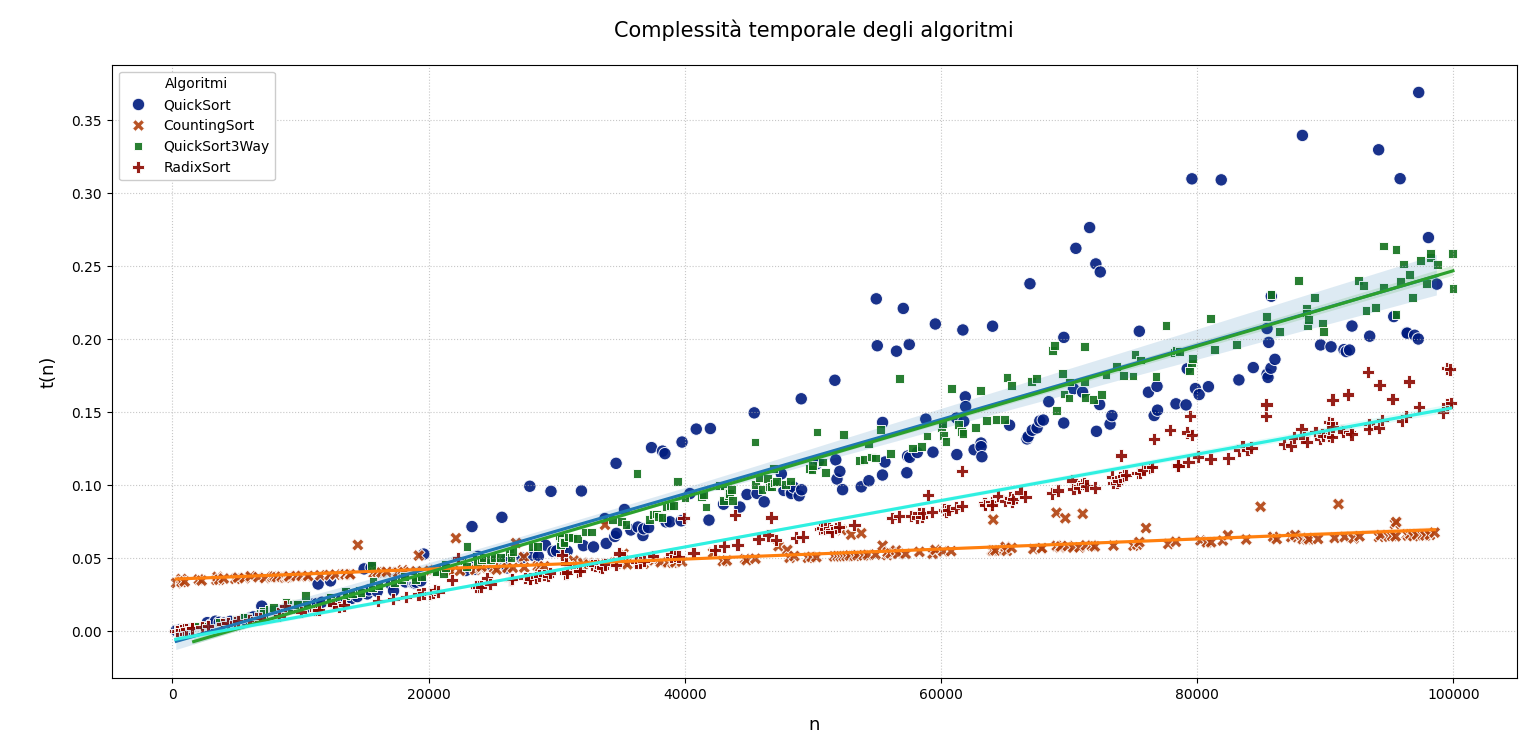
\includegraphics[scale=0.5]{Immagini/Grafico.png}
    \caption*{Parte reale sulle x, parte immaginaria sulle y}
\end{figure}

\section{Conclusioni}

\paragraph{Sintesi dei risultati.}
Gli esperimenti condotti confermano le attese teoriche sulle famiglie di algoritmi considerate. 
Tra gli algoritmi \emph{comparativi}, \texttt{QuickSort} e \texttt{QuickSort 3-way} presentano tempi che, al crescere della dimensione dell'input \(n\), sono compatibili con una complessità \(O(n\log n)\), mentre un algoritmo quadratico di riferimento (se considerato) degrada rapidamente. 
Tra gli algoritmi \emph{non comparativi}, \texttt{Counting Sort} e \texttt{Radix Sort} evidenziano i loro punti di forza: il primo è lineare in \(n\) quando il range dei valori \(m\) è moderato (complessità \(O(n+m)\) e spazio \(O(m)\)), il secondo è efficace quando le chiavi hanno lunghezza fissa (complessità \(\Theta(d(n+k))\) con \(d\) numero di cifre e \(k\) la base/bucket), risultando poco sensibile a \(m\) se \(d\) rimane contenuto.

\paragraph{Validazione empirica.}
I grafici in scala log--log (tempo vs \(n\) e tempo vs \(m\)) hanno fornito una verifica quantitativa: 
le pendenze stimate per \texttt{QuickSort}/\texttt{QuickSort 3-way} sono prossime a \(1\) (coerenti con \(n\log n\) su intervalli finiti), 
quelle di \texttt{Counting Sort} rispetto a \(m\) sono vicine a \(1\) (costo di inizializzazione dell'array dei contatori), 
e il \emph{caso peggiore} di \texttt{QuickSort} su input ordinato mostra un comportamento compatibile con \(O(n^2)\) (pendenza prossima a \(2\)). 
Le barre d'errore ridotte indicano stabilità delle misure; eventuali variazioni localizzate sono attribuibili al rumore di sistema e alla generazione degli input.

\paragraph{Trade-off pratici.}
Oltre all'ordine asintotico, emergono differenze concrete dovute a costanti e gestione della memoria. 
\texttt{QuickSort} è tipicamente il più rapido in media e in-place (stack atteso \(O(\log n)\)), ma non è stabile e può degradare se la scelta del pivot è sfavorevole; tecniche come pivot randomizzato, median-of-three e partizionamento 3-way riducono drasticamente tale rischio. 
\texttt{QucikSort3Way} offre prestazioni prevedibili, è stabile e adatto a flussi/esterni, ma richiede spazio addizionale \(O(n)\). 
\texttt{Counting Sort} è stabilmente lineare quando \(m=O(n)\), ma lo spazio \(O(m)\) ne limita l'uso per range molto ampi. 
\texttt{Radix Sort}, usando una routine stabile (ad es. \texttt{Counting Sort}) come subprocedura, scala bene su chiavi a lunghezza fissa, con costi che dipendono da \(d\) più che da \(m\).

\paragraph{Linee guida operative.}
\begin{itemize}
  \item \textbf{Uso generale su chiavi generiche:} preferire \texttt{QuickSort} con pivot robusto (random/median-of-three) o \texttt{MergeSort} quando serve stabilità.
  \item \textbf{Molte duplicazioni:} \texttt{QuickSort 3-way} riduce il lavoro sui segmenti di uguali.
  \item \textbf{Chiavi intere in range moderato:} \texttt{Counting Sort} è ideale (tempo \(O(n+m)\), stabile), purché la memoria \(O(m)\) sia sostenibile.
  \item \textbf{Chiavi a lunghezza fissa/byte-string:} \texttt{Radix Sort} è competitivo e poco sensibile a \(m\), specialmente con base e \(d\) scelti con cura.
\end{itemize}

\paragraph{Limiti e minacce alla validità.}
Le misure dipendono dall'hardware, dal sistema operativo, dalla gestione del \emph{runtime} e dalla distribuzione degli input. 
Sebbene si siano effettuate più ripetizioni e si siano usate scale logaritmiche per mitigare l'effetto del rumore e stimare gli esponenti, restano possibili bias dovuti a cache, branch prediction, allocazioni di memoria e dettagli implementativi. 
I risultati vanno letti come conferme sperimentali \emph{coerenti} con la teoria, non come stime assolute universalmente trasferibili.

\paragraph{Conclusione finale.}
In sintesi, l'analisi congiunta teorico--sperimentale mostra che:
(i) gli algoritmi comparativi ben progettati (\texttt{QuickSort} con scelte di pivot robuste e \texttt{MergeSort}) sono la scelta predefinita su input generici grazie a prestazioni \(O(n\log n)\) affidabili; 
(ii) in scenari strutturati, gli algoritmi non comparativi (\texttt{Counting}/\texttt{Radix}) offrono vantaggi decisivi, purché le ipotesi (\(m\) moderato, chiavi a lunghezza fissa, stabilità della subroutine) siano soddisfatte; 
(iii) la selezione dell'algoritmo deve considerare non solo l'asintotica, ma anche stabilità, consumo di memoria e caratteristiche del dominio dei dati. 
Questi risultati forniscono un criterio pratico per scegliere consapevolmente l'algoritmo più adatto al contesto applicativo.


\end{document}